
\documentclass[12pt]{article}
\usepackage{titlesec}
\usepackage[utf8]{inputenc}
\usepackage[T1]{fontenc}
\usepackage[english]{babel}

\usepackage{graphicx}
\graphicspath{{images/}}
\usepackage{float}

\usepackage{diagbox}

\usepackage{natbib}
\bibliographystyle{agsm}  


\usepackage[hidelinks]{hyperref}  

\usepackage{amsmath} 
\usepackage{amsfonts}
\usepackage{amssymb}

\usepackage[a4paper, width=150mm, top=25mm, bottom=25mm]{geometry}
\usepackage{pdflscape}
\usepackage{pdflscape}
\usepackage{everypage}
\usepackage{lipsum}
\usepackage{rotating}
\usepackage{setspace}
\usepackage{fancyhdr}
\pagestyle{fancy}
\newcolumntype{L}{>{\raggedright\arraybackslash}m{10cm}}

\newcommand{\Lpagenumber}{\ifdim\textwidth=\linewidth\else\bgroup
  \dimendef\margin=0 %use \margin instead of \dimen0
  \ifodd\value{page}\margin=\oddsidemargin
  \else\margin=\evensidemargin
  \fi
  \raisebox{\dimexpr -\topmargin-\headheight-\headsep-0.5\linewidth}[0pt][0pt]{%
    \rlap{\hspace{\dimexpr \margin+\textheight+\footskip}%
    \llap{\rotatebox{90}{\thepage}}}}%
\egroup\fi}
\AddEverypageHook{\Lpagenumber}%

\usepackage[ruled,vlined]{algorithm2e}
\SetAlCapNameFnt{\scriptsize}
\SetAlCapFnt{\scriptsize}
\newlength\mylen
\newcommand\myinput[1]{%
  \settowidth\mylen{\KwIn{}}%
  \setlength\hangindent{\mylen}%
  \hspace*{\mylen}#1\\}

% \titleformat{\chapter}[display]
% {\normalfont\bfseries}{}{0pt}{\Huge}
 

\begin{document}
  
  \begin{titlepage}
    \begin{center}
      \vspace{1em}
	  \large{Master Thesis}\\
	  \huge Gaining Customer Insights using Machine Learning on Graphs \\ 
	  \large \vspace{1em}
	  University of Basel\\
	  \vspace{4em} 
	  \large
	  Author: \\
	  Michael von Siebenthal\\
	  \vspace{2em}
	  Supervisor: \\
	  Prof. Dr. Dietmar Maringer\\
	  \vspace{2em}
	  \today
	  \vspace{3em}
    \end{center}
  \end{titlepage} 



  %%% frontmatter
  \section*{Abstract}

This is the abstract.

  
    "I hereby declare - that I have written this master thesis without any help 
  from others and without the use of documents and aids other than those stated 
  in the references, - that I have mentioned all the sources used and that I 
  have cited them correctly according to the established academic citation rules, 
  - that the topic or part of it are not already the object of any work or 
  examination of another course unless explicitly stated,- that I am aware of 
  the consequences of plagiarism at the Business and Economics Faculty of University of Basel."\\\\\\\\\\
  Michael von Siebenthal, Martikel-Nr.: 2015-256-837, Date: \today

  %  "I hereby declare - that I have written this master thesis without any help 
  from others and without the use of documents and aids other than those stated 
  in the references, - that I have mentioned all the sources used and that I 
  have cited them correctly according to the established academic citation rules, 
  - that the topic or part of it are not already the object of any work or 
  examination of another course unless explicitly stated,- that I am aware of 
  the consequences of plagiarism at the Business and Economics Faculty of University of Basel."\\\\\\\\\\
  Michael von Siebenthal, Martikel-Nr.: 2015-256-837, Date: \today


  \tableofcontents
  \listoffigures
  \listoftables

  %%% Main Body
  \onehalfspacing
  
  % Introduction
  	
	This thesis investigates models for gaining customer insights using graph
	machine learning. Graph machine learning is a current frontier in machine 
	learning and has many successful applications in many areas such as recently 
	shown by the success of AlphaFold \citep{senior2020improved}. AlphaFold made 
	a breakthrough for predicting protein structures where they made use of the 
	observation that a folded protein can be considered as a spatial graph 
	\citep{AlphaFoldTeam2020}. More generally, there are a vast range of 
	applications for graph machine learning in the fields of natural science, 
	social science and many more as shown by the excellent overview given by 
	\cite{zhou2020graph}. Graphs are especially useful as they allow for the 
	consideration of relationships between observations. Graph machine learning 
	has for that reason become a promising field as it allows for the use of
	richer data. This thesis will focus on graph machine learning for the
	purpose of customer classification. In particular, it is investigated to
	what extent semi-synthetic graphs can be used for graph machine learning.
	To provide a better overview as to how this topic relates to business \& 
	economics related fields such as gaining customer insights, some motivating
	examples are provided in the following section. 
	
	\section{Relevance to Economics}

	\noindent From a business \& economics perspective, graphs are particularly
	interesting if one wants to model the interactions between institutions. An 
	example for this is shown in an article published by 
	\cite{schweitzer2009economic} which created the graph shown in figure
	\ref{fig:bank_network}. This graph depicts the interdependencies of 
	international banks. Such graphs can be useful tools for analyzing such 
	interdependencies and to provide important information for making the banking 
	system more robust and resilient. 

	\begin{figure}[h]
		\centering
		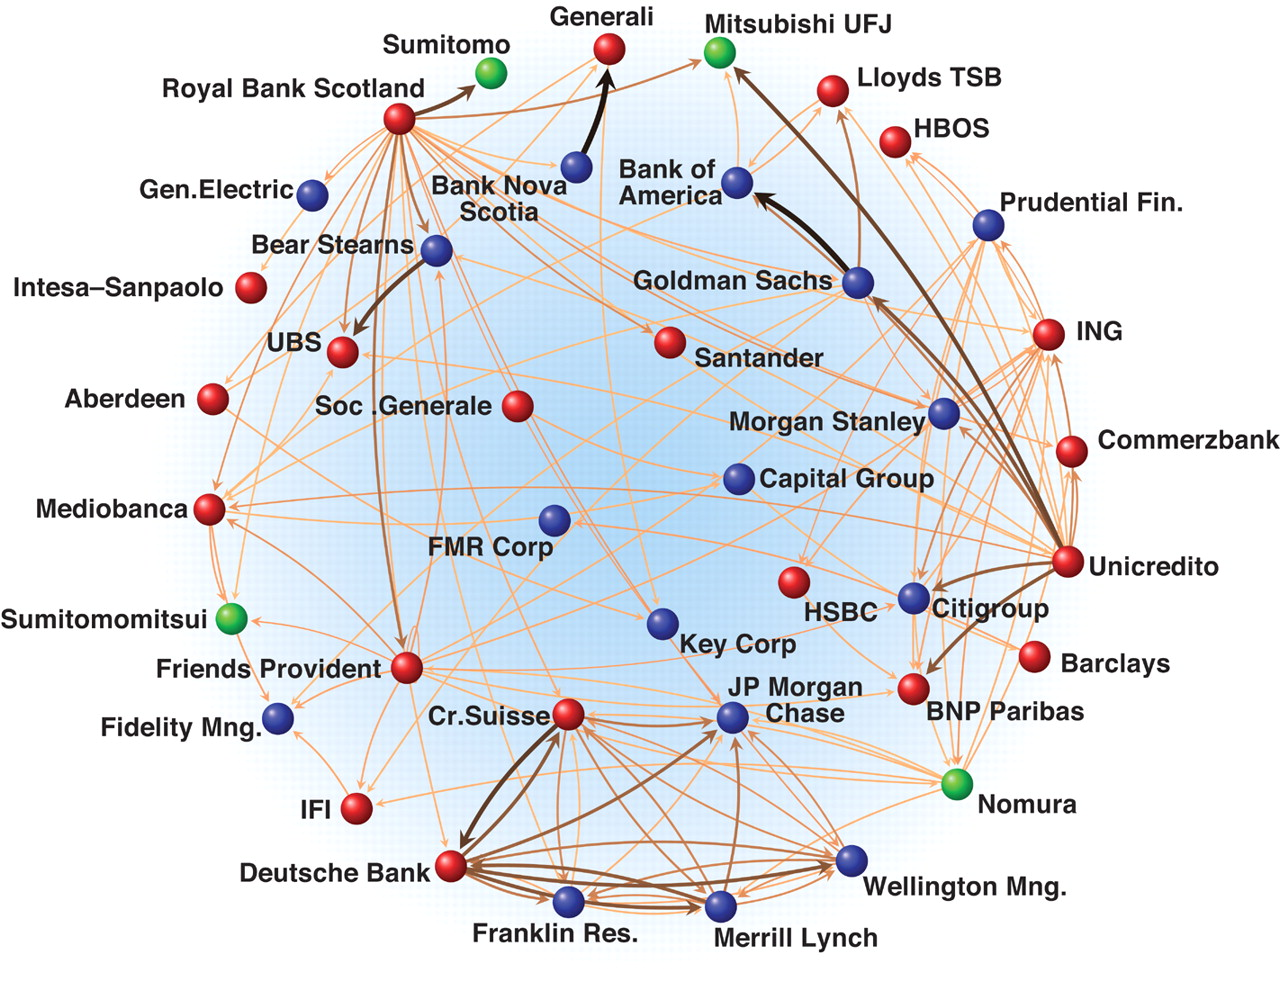
\includegraphics[width=0.5\textwidth]{bank_network.jpg}
		\caption{Bank Network}
		\cite[p. 424]{schweitzer2009economic}
		\label{fig:bank_network}
	\end{figure} 

	\noindent Another interesting application of graphs is to model social 
	interactions. While there are many different areas of interest which make
	use of social connections, the focus of this thesis is placed on gaining 
	customer insights. Indeed, this is one of the main areas where social network 
	companies such as Facebook or search providers like Google make their
	revenue. Those companies mainly generate their revenue by providing customer 
	insights or selling targeted advertising \citep{Facebook2021,Alphabet2021}. 
	Both Facebook and Google have the advantage, that their businesses naturally 
	capture relational or more generally network data. Most researchers and 
	companies however do not have access to such data. Companies for instance 
	may have access to large amounts of customer data. This data however 
	typically does not contain relational information (e.g. which client is 
	connected with which other clients). The same is true for researchers, where 
	social scientists often collect data via anonymous surveys. This makes the 
	collection of network data basically impossible. For that reason, most 
	companies and researchers are limited to working with data such as 
	cross-sectional data that contain no network information. It is important 
	to mention, that there is a lot of network data available online. This 
	network data however typically only contains the network connections. The 
	important feature data such as demographic data, topic specific variables 
	and labels are however typically not available. Without feature data, graphs 
	provide rather limited information for gaining customer insights. 
	This is a data access and data collection problem and is a frustrating 
	reality which also affects this master's thesis. It however motivates the 
	research topic which is presented in section \ref{section:research_topics}. 
	First, a general overview of machine learning is given in the following 
	section.
	
	\section{Overview Machine Learning}

	This section provides a high-level overview of machine learning and
	specifies the type of machine learning task used for this thesis. To
	start, it is important to correctly categorize machine learning. There are
	many related big topics such as data science, big data or artificial
	intelligence and it is often not clear what exactly is meant. An overview
	of how these different terms can be categorized is shown in figure 
	\ref{fig:ml_overview}.

	\begin{figure}[h]
		\centering
		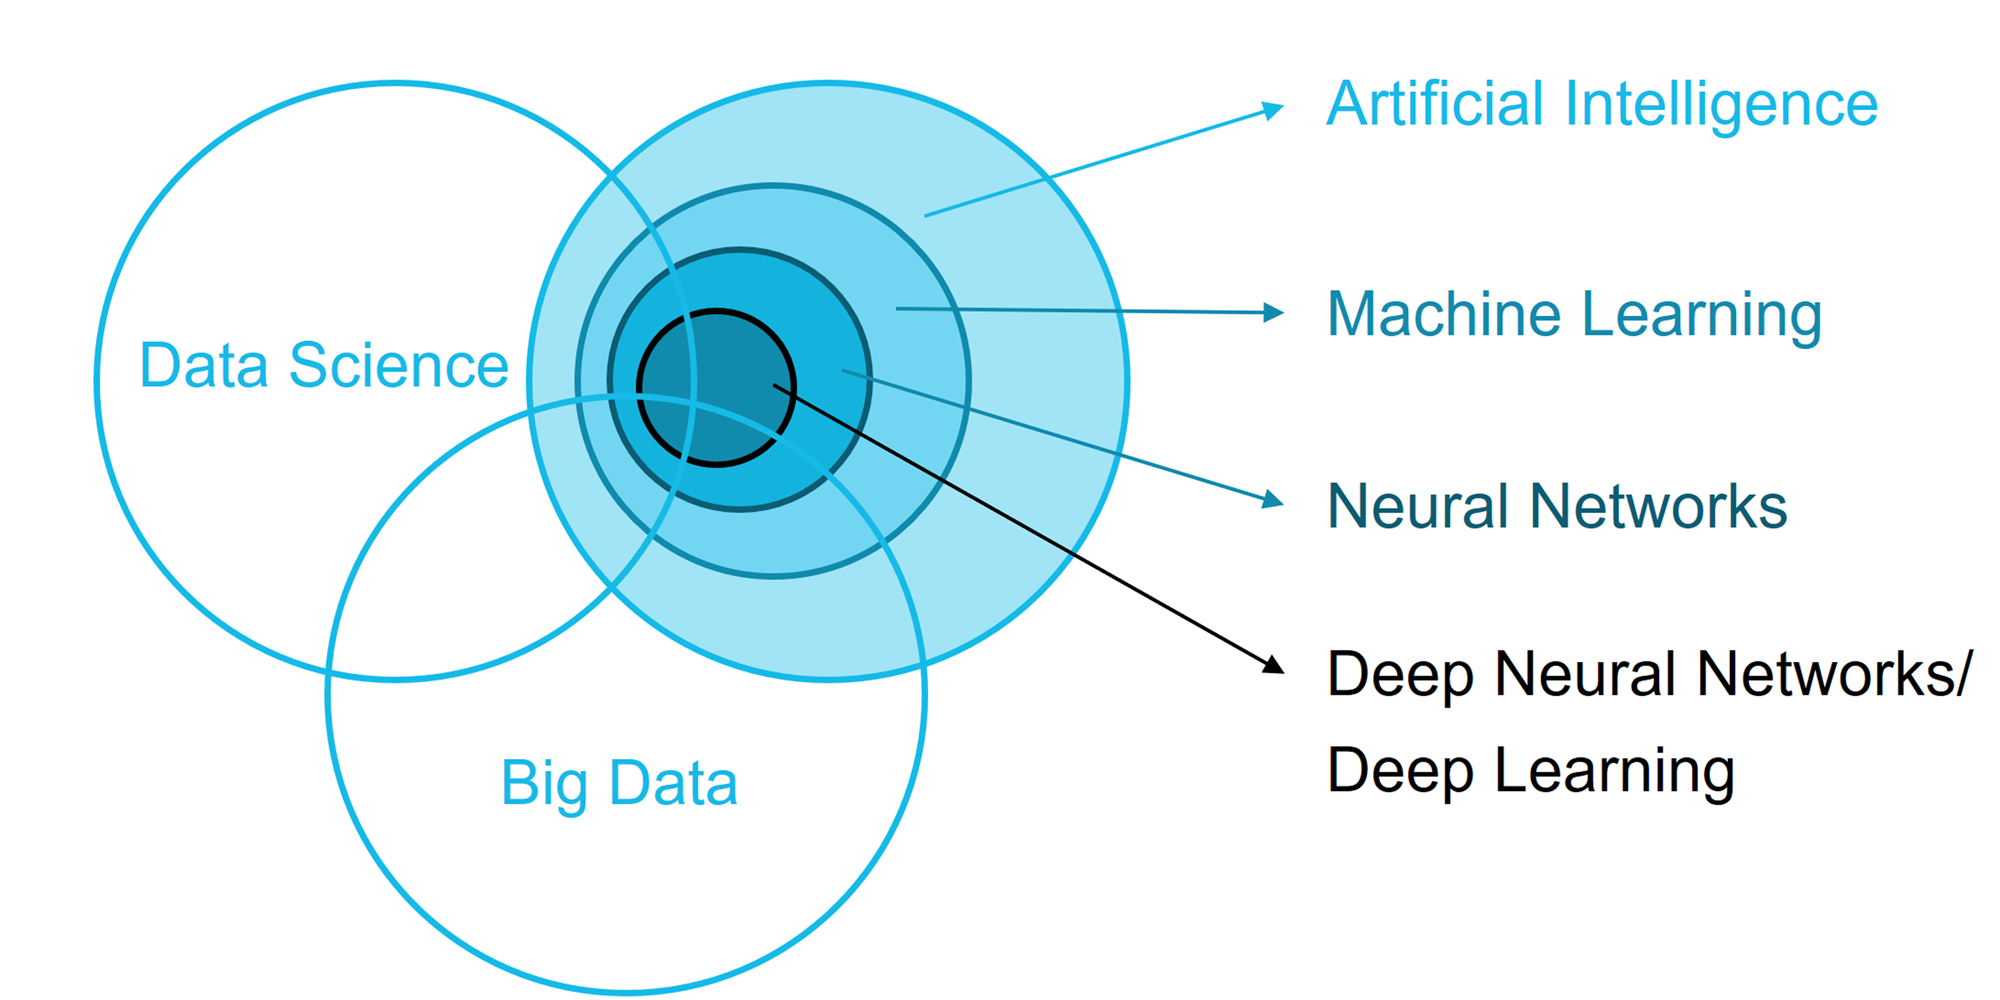
\includegraphics[width=0.7\textwidth]{overview_datascience.png}
		\caption{Overview Machine Learning}
		\citep{Frauenhofer2021}
		\label{fig:ml_overview}
	\end{figure} 

	\noindent Figure \ref{fig:ml_overview} shows well, how these different
	terms are related with each other. Machine learning in particular is
	mostly ascribed to the domain of artificial intelligence. It however also 
	has a shared domain with data science and big data. It is thus at the
	intersection of these three interrelated fields. Machine learning models 
	such as neural networks and deep neural networks are specific models within
	machine learning and are often referred to separately due to their
	popularity. In this thesis, differentiating between machine learning and
	neural networks is not necessary, as the considered machine learning models
	are used for the same task. Machine learning can be applied for various
	tasks and is again best presented visually as shown in figure 
	\ref{fig:ml_tasks}.

	\begin{figure}[h]
		\centering
		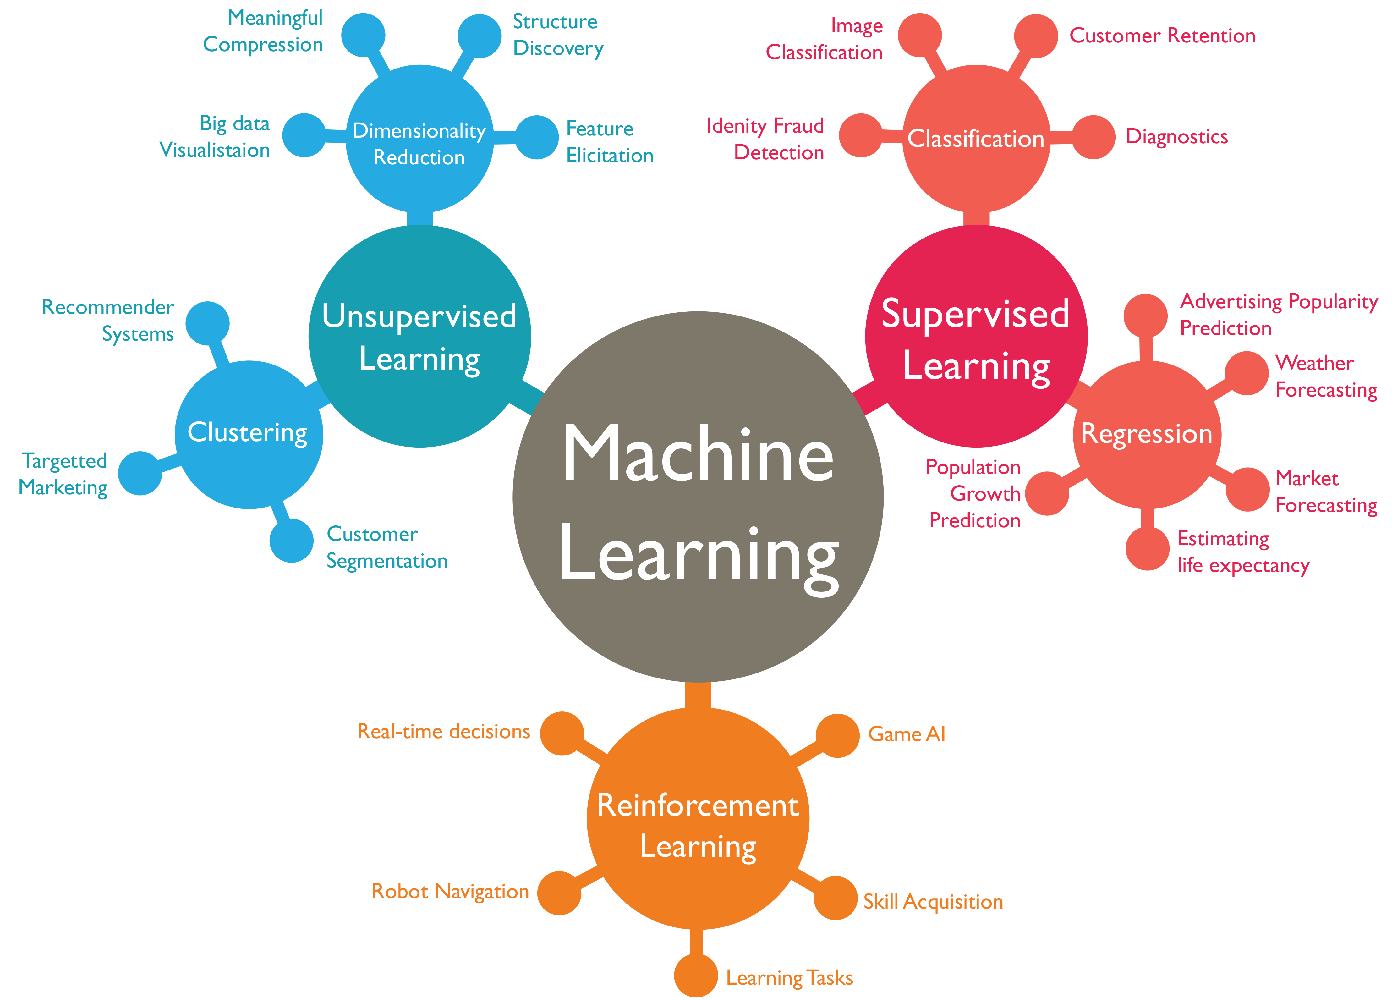
\includegraphics[width=0.8\textwidth]{ml_tasks.png}
		\caption{Overview Machine Learning Tasks}
		\citep{Artisan2020}
		\label{fig:ml_tasks}
	\end{figure} 

	\noindent It is shown in figure \ref{fig:ml_tasks}, that the main tasks for
	machine learning involve classification, regression, reinforcement
	learning, clustering and dimensionality reduction. This thesis focuses on 
	classification tasks. This task is chosen given the available data and 
	because it allows for a nice comparison of different machine learning models. 
	Well known standard machine learning models used for classification tasks 
	include logistic regression \citep{cramer2002origins}, naive bayes 
	\citep{zhang2004bayes}, support vector machines 
	\citep{platt1999probabilistic}, random forest classifiers
	\citep{breiman2001random}, AdaBoost \citep{freund1997decision} and
	artificial neural networks \citep{mcculloch1943logical}. This is an
	incomplete list of popular machine learning models that can be used for
	classification tasks. Popular applications of classification tasks include 
	predicting whether a customer is satisfied, whether to grant a mortgage 
	to a client and many more. The aforementioned machine learning methods have 
	in common, that they all only consider feature data and cannot consider 
	network information. \\

	\noindent Graph machine learning methods are different in that they consider 
	both feature data as well as network information. If one wants to categorize 
	graph machine learning within the framework shown in figure 
	\ref{fig:ml_overview}, it is probably best categorized as a special form of 
	neural network. It is however not a deep neural network, as network depth 
	does not necessarily improve the model and can be even counter-productive. 
	Within graph machine learning, there are two main approaches. The first 
	approach focuses on learning vector representations of graphs which are 
	used for downstream machine learning. The downstream machine learning models 
	include the standard models presented previously. Graph representation 
	learning approaches include models such as DeepWalk 
	\citep{perozzi2014deepwalk} and Node2Vec \citep{grover2016node2vec} among 
	others. The second approach involves the application of graph neural 
	networks for which there exist many different models. These networks 
	include models such as Graph Convolutional Networks \citep{kipf2016semi}, 
	GraphSage \citep{hamilton2017inductive} and many more. \\

	\noindent The detailed theoretical background for the considered graph
	machine learning models is provided in chapter 2.

	\section{Research Topic}
	\label{section:research_topics}

	\noindent The difficult access to graphs which also contain features, 
	motivate the search for alternatives. A review of the literature revealed, 
	that a form of synthetic graph generation could provide a solution to the data 
	access problem. Classic graph generation procedures include the famous 
	Erdös-Rényi graphs \citeyearpar{erdos1959random}, the small-world model by 
	\cite{watts1998collective}, the well-known model by 
	\cite{barabasi1999emergence} and more recently Kronecker Graphs by
	\cite{leskovec2010kronecker}. These models are all very instructive
	regarding the graph generation process and for understanding graph
	properties. These networks however all have the short-coming, that they do 
	not allow for the assignment of feature data to the nodes/observations in the
	network. It became clear, that one has to find or develop a model which 
	makes use of existing feature data for the graph generation process. 
	\cite{kim2012multiplicative} developed the \ac{mag} model. This model makes 
	use of randomly generated feature data which is referred to as attribute data 
	by the authors. The model is shown to be capable of generating random graphs 
	which can adhere to observed real world network properties. An analysis of 
	the \ac{mag} model reveals, that it could also be a useful model for 
	creating semi-synthetic graphs using existing feature data. For that reason, 
	the \ac{mag} model is selected for generating semi-synthetic graphs. This 
	model is introduced in detail in section \ref{section:theory_graphgen}. \\

	\noindent More recently, researchers have focused their attention to
	generative graph models. These models create graphs with features using
	real graphs as a training input. Examples for such models are graph
	\ac{rnn} \citep{you2018graphrnn} and deep generative graph
	models \citep{li2018learning}. These are very fascinating models which can
	be used to recreate or scale graph data. For the purpose of this thesis,
	these models are not purposeful, as it requires an existing graph with
	features to be available. Such a graph is unfortunately not available for
	this thesis. Nevertheless, this is an interesting current topic for graph 
	generation which was considered. \\ 

	\noindent The access problem to graphs which include feature data might be 
	resolved using the \ac{mag} model as previously mentioned. This model is 
	interesting as most researchers and companies have access to large amounts 
	of feature data such as customer databases or survey data. It would be of
	great benefit, if the available feature data could be used for generating
	semi-synthetic graphs. The \acs{mag} model provides a solution for
	generating such graphs. Semi-synthetic graph refers to the fact, that the 
	graph is generated using real feature data. Fully synthetic graphs on the 
	other hand are generated exclusively using artificial data. The goal of the
	semi-synthetic graph is to generate connections between the observations in 
	a given dataset. These connections should enhance the information present
	in the dataset. Graph machine learning should then be capable of exploiting
	these additional connections and hopefully provide competitive if not
	superior results compared to standard machine learning models. This thesis 
	therefore investigates to what extent semi-synthetic graphs can be used for 
	graph machine learning. Of course, semi-synthetic graphs are unlikely to be
	capable of fully substituting the performance of real graphs for machine 
	learning. Nevertheless, semi-synthetic graphs provide additional and 
	hopefully useful network information. To assess these hypotheses, the 
	results using graph machine learning are compared to standard machine 
	learning models. To close this section, the research question as well as the 
	hypotheses of this thesis are presented formally as follows. 

	\paragraph{Research Question}\mbox{}

	\noindent To what extent are semi-synthetic graphs based on real 
				feature data useful for a classification task using machine
				learning?

	\paragraph{Hypotheses}\mbox{}

	\noindent\textbf{H1:} Graph machine learning using semi-synthetic graphs
	provide superior results compared to the results of standard machine
	learning for a given classification task.\\

	\noindent\textbf{H2:} Graph machine learning using semi-synthetic graphs is
	a competitive strategy compared to the results of standard machine
	learning for a given classification task.\\


	\noindent The required theoretical background for this thesis which
	includes graph machine learning, graph generation and graph theory in
	general is provided in chapter 2.



  % Theory
  
	This chapter covers the required theoretical background and consists 
	of the following main parts:

	\begin{enumerate}
		\item Graph Theory
		\item Machine Learning on Graphs
		\item Graph Generation
    \end{enumerate}

	\section{Graph Theory}

	This section provides a brief introduction to graph theory with a focus on
	the relevant aspects for this master's thesis. The theory presented is
	primarily taken from the book "Networks: An Introduction" by Mark Newman
	\citeyearpar{Newman2010}. \\

	\noindent Graph theory is an old field of mathematics and can be traced back 
	to Leonhard Euler and the famous "Königsberg Bridge Problem"
	\citep{euler1741solutio}. The study of graphs has had a recent revival
	thanks to its useful applications in areas such as the Google algorithm
	PageRank \cite{page1999pagerank} and graph machine learning. Graphs are 
	special data structures as shown in Figure \ref{fig:graph}. The terms graph 
	and network are often used interchangeably and have the identical meaning 
	for the purpose of this master's thesis. Typically, the term graph is used 
	more commonly for the mathematical analysis of graphs and the term network 
	is more commonly used for data science purposes. \\

	\begin{figure}[h]
		\centering
		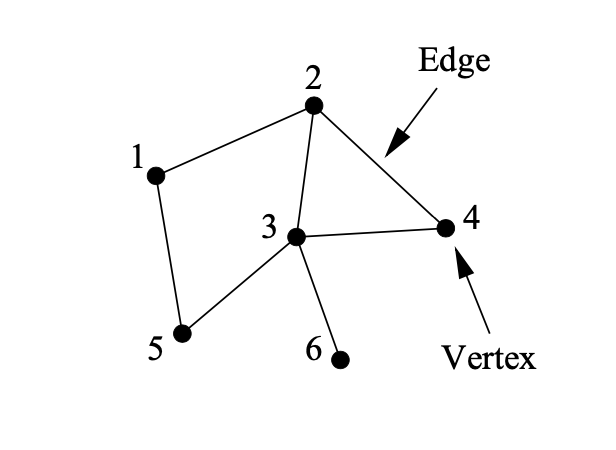
\includegraphics[width=0.5\textwidth]{graph.png}
		\caption{Example of a Graph}
		\cite[p. 111]{Newman2010}
		\label{fig:graph}
	\end{figure}
	
	\noindent The graph shown in Figure \ref{fig:graph} corresponds to an 
	undirected graph in which the connections between the vertices are mutual. 
	In a directed graph for instance, vertex A could be connected to vertex B, 
	however vertex B need not be connected to vertex A. For the purpose of this 
	thesis, only undirected graphs are considered. Vertices are often referred 
	to as nodes and the terms are used interchangeably. Edges refer to the
	connections between the vertices. Edges are often also referred to as links
	and the terms are used interchangeably as well. Graphs may have additional 
	elements such as multi-edges or self-edges. Self-edges refer to
	nodes which have a looped link to themselves. This can be considered as a
	form of feedback loop of a node on to itself. Lastly, multi-edges refer to 
	direct node connections with multiple paths. \\

	\noindent For mathematical notation, graphs are typically defined as follows:

	\begin{equation}
		G(V,E)
	\end{equation}

	\noindent $G$ denotes the graph. $V$ refers to the set of vertices present 
	in the graph and $E$ refers to edges present between the vertices.

	\paragraph{Adjacency Matrix} \mbox{}\\  

	\noindent The adjacency matrix $A$ is defined as a $N \times N$ matrix, 
	where $N$ refers to the number of vertices present in the graph. Each 
	vertex is therefore recorded by a column and a row in the adjacency matrix. 
	The elements in the adjacency matrix are further typically defined as follows:

	\begin{equation}
		A_{ij} = 
			\begin{cases}
				1, & \text{if vertex $i$ and $j$ are connected by an edge} \\
				0, & \text{otherwise}
			\end{cases}
	\end{equation}
	
	\noindent For illustration, the adjacency matrix of the graph shown in 
	Figure \ref{fig:graph} is shown as follows:

	\[ A = 
	\begin{pmatrix}
		0 & 1 & 0 & 0 & 1 & 0 \\
		1 & 0 & 1 & 1 & 0 & 0 \\
		0 & 1 & 0 & 1 & 1 & 1 \\
		0 & 1 & 1 & 0 & 0 & 0 \\
		1 & 0 & 1 & 0 & 0 & 0 \\
		0 & 0 & 1 & 0 & 0 & 0  
	\end{pmatrix}
	\] 
	
	\noindent As one can see, if vertex $i$ and $j$ are connected, this is 
	recorded with 1 and 0 otherwise. Note, that all the elements on the 
	$diag(A)$ are equal to 0. This is because there are no self-edges present 
	in figure \ref{fig:graph}. Nodes with self-loops would have a 1 recorded on 
	the corresponding diagonal element of the adjacency matrix. As this is an 
	undirected network, the adjacency matrix is symmetric. There are many 
	additional aspects one could mention with regard to the adjacency matrix, 
	they are however not relevant for this thesis. For additional information 
	regarding the adjacency matrix, the book "Networks: An Introduction" by 
	Mark Newman \citeyearpar{Newman2010} is highly recommended. 

	\paragraph{Degree Measures} \mbox{}\\

	\noindent An important measure for graphs are the degrees denoted by $k$ of 
	the vertices. Degrees refer to the number of edges connected to a vertex. The 
	degrees of vertex denoted by $i$ can be formulated as \citep[p. 133]{Newman2010}:

	\begin{equation}
		k_i = \sum_{j=1}^{n} A_{ij}
	\end{equation}

	\noindent For an undirected graph, edges have two ends. This is due to the 
	fact that vertices connected by an edge are mutually connected. In terms of 
	the sum of the degrees of all vertices, we can therefore write for an
	undirected graph with $m$ edges \citep[p. 133]{Newman2010}:

	\begin{equation}
		2m = \sum_{i=1}^{n} k_i	
	\end{equation}

	\noindent As a statistical measure, the mean degree $c$ of a vertex is 
	defined as follows \citep[p. 134]{Newman2010}:

	\begin{equation}
		c = \frac{1}{n}\sum_{i=1}^{n}k_i = \frac{2m}{n}
	\end{equation}

	\noindent To calculate the density of a graph, it should first be noted, 
	that the maximum number of edges is given by \citep[p. 134]{Newman2010}:

	\begin{equation}
		{n \choose 2} = \frac{1}{2}n(n-1)
	\end{equation}

	\noindent The density $\rho$ can thus be written as \citep[p. 134]{Newman2010}:

	\begin{equation}
		\rho = \frac{m}{{n \choose 2}} = \frac{2m}{n(n-1)} = \frac{c}{n-1}
	\end{equation}

	\noindent Note, that the density $\rho$ lies strictly between 
	$0 \leqslant \rho \leqslant 1$. In addition, for sufficiently large graphs,
	one can approximate $\rho = \frac{c}{n}$. 

	\paragraph{Eigenvector Centrality} \mbox{}\\

	\noindent The degrees of a vertex shown in the previous section correspond 
	to the simplest form of a centrality measure. The issue with this measure 
	is, that the every neighbor of vertex $i$ is valued the same. This is a 
	problem, as not all neighbors are of equal importance due to the:

	\begin{enumerate}
		\item Number of neighbors
		\item Importance of neighbors
		\item Both
	\end{enumerate}

	\noindent There are many different alternative centrality measures which
	can consider the factors listed above such as eigenvector centrality, Katz
	centrality or PageRank
	\citep{katz1953new,page1999pagerank,landau1895relativen,Newman2010}. As
	this thesis only considers simple undirected graphs, eigenvector centrality 
	will suffice. \\

	\noindent Eigenvector centrality gives all vertices a score which is 
	proportional to the sum of the scores of the vertices neighbors. This is a 
	procedure in which typically the initial centrality $x_i$ of vertex $i$ is 
	guessed to be 1, $\forall i$. This can be used to calculate the 
	centralities of the neighbors of $i$ which is denoted as $x_{i}'$. One can 
	thus write \citep[p. 169]{Newman2010}:

	\begin{equation}
		x_i' = \sum_{j}A_{ij}x_j
	\end{equation}

	\noindent In matrix notation:

	\begin{equation}
		x' = Ax
	\end{equation}

	\noindent This process is repeated $t$ times as follows to generate better 
	estimates \citep[p. 170]{Newman2010}:

	\begin{equation}
		x(t) =  A^tx(0)
	\end{equation}

	\noindent $x(0)$ denotes the linear combination of 
	\citep[p. 170]{Newman2010}:

	\begin{equation}
		x(0) =  \sum_{i}c_{i}v_{i}
	\end{equation}

	\noindent $v_i$ corresponds to the eigenvectors of the adjacency matrix $A$
	and $c_i$ corresponds to an appropriately chosen constant. Therefore one can
	write \citep[p. 170]{Newman2010}:

	\begin{equation}
		x(t) =  A^t \sum_{i}c_{i}v_{i} = \sum_{i} c_i k_i^t v_i = 
		k_i^t \sum_{i} c_i \left[\frac{k_i}{k_1}\right]^t v_i
		\label{eq:eigenvec_cent}
	\end{equation}

	\noindent In equation \ref{eq:eigenvec_cent}, $k_i$ correspond to the 
	eigenvalues of the adjacency matrix $A$. $k_1$ corresponds to the largest 
	eigenvalue of $A$. As $\frac{k_i}{k_1} < 1, \; \forall \; i\neq 1$ , the 
	term is decaying as $t \rightarrow \infty$. The centralities $x$ can 
	therefore be written in terms of fulfilling following condition 
	\citep[p. 170]{Newman2010}:

	\begin{equation}
		Ax = k_1 x	
	\end{equation}

	\noindent Lastly, the eigenvector centrality is defined as \citep[p. 170]{Newman2010}:

	\begin{equation}
		x_i = k_{1}^{-1} \sum_{j} A_{ij}x_j 
	\end{equation}

	\paragraph{Closeness Centrality} \mbox{}\\

	\noindent Closeness centrality, $C_i$, is defined as the average distance 
	of a vertex to the other vertices in the graph. This centrality measure is 
	defined as follows \citep[p. 182]{Newman2010}:

	\begin{equation}
		C_i = \frac{1}{l_i} = \frac{n}{\sum_{j}d_{ij}}
	\end{equation}

	\noindent For this measure, central vertices exhibit high closeness 
	centrality and are therefore more closely connected to other vertices 
	compared to vertices with low closeness centrality. $l_i$ refers to the 
	average of the geodesic distances $d_{ij}$ of vertex $i$.

	\paragraph{Betweenness Centrality} \mbox{}\\

	\noindent This centrality measures to which extent a vertex lies on paths 
	between other vertices. For instance, a bottle neck vertex would exhibit a 
	large betweenness centrality as many, if not all nodes must pass through it. 
	More formally, betweenness centrality $x_i$ is defined as 
	\citep[p. 187]{Newman2010}:

	\begin{equation}
		x_i = \sum_{st} \frac{\eta_{st}^i}{g_{st}}
		\label{eq:between_cent}
	\end{equation}

	\noindent In equation \ref{eq:between_cent}, $\eta_{st}^i$ refers to the 
	number of geodesic paths from $s$ to $t$ which pass through vertex $i$. 
	Further, $g_{st}$ is defined as the number of geodesic paths between vertex 
	$s$ and $t$. \\

	\noindent In order to allow for better comparison of betweenness
	centralities, it is often standardized by the number of connected vertex
	pairs $s$ and $t$ denoted as  $\eta^2$. The betweenness centrality
	can therefore be rewritten as \citep[p.190]{Newman2010}:

	\begin{equation}
		x_i = \frac{1}{\eta^2}\sum_{st} \frac{\eta_{st}^i}{g_{st}}
	\end{equation}

	\noindent With this measure, the betweenness centrality is within the range
	$0\leqslant1$.

	\section{Machine Learning on Graphs}

	\noindent Graph structures are special in that the data points in a graph 
	have connections with each other. A practical example for this are social 
	networks. In a social network, the profiles of "Peter" and "Paul" might be 
	connected because "Peter" and "Paul" are friends. In addition, "Paul" and 
	"Peter" can only ever reach each-other if they are directly or perhaps 
	indirectly connected via a mutual friend. This aspect is unique to network 
	data and provides interesting additional information as well as added
	complexity. This property does not allow for comparing nodes in a graph in 
	terms of euclidean distances as only connected nodes can reach each-other.
	For that reason, graphs cannot be directly plotted as scatter plots since
	standard distance measures cannot be directly applied to determine node 
	similarities. The graph machine learning methods used for this thesis can 
	be categorized into the following two categories:

	\begin{enumerate}
		\item Graph Representation Learning
		\item Graph Neural Networks
	\end{enumerate}
	
	\noindent Graph representation learning refers to models which generate node
	embeddings of a given graph. Specifically, this approach creates vector 
	representations of the nodes in a graph given a specified similarity measure. 
	For these vector representations distance measures such as Euclidean 
	distances can be measured. The node embeddings can thus be used for
	downstream machine learning using standard methods. Graph neural networks 
	can also generate node embeddings as well as directly applying graphs to a 
	given machine learning task such as classification. The capability of
	directly applying graphs for machine learning tasks, makes graph neural 
	networks especially promising. \\

	\noindent In the following subsections, the theory for graph representation 
	learning and graph neural networks is introduced. 

	\subsection{Graph Representation Learning}

	The aim of graph representation learning is to generate node embeddings in 
	the form of $d$-dimensional vector representations. The resulting node 
	embeddings can then be used for "standard" machine learning applications. 
	A graphical representation of this task is shown in figure 
	\ref{fig:embedding}.

	\begin{figure}[h]
		\centering
		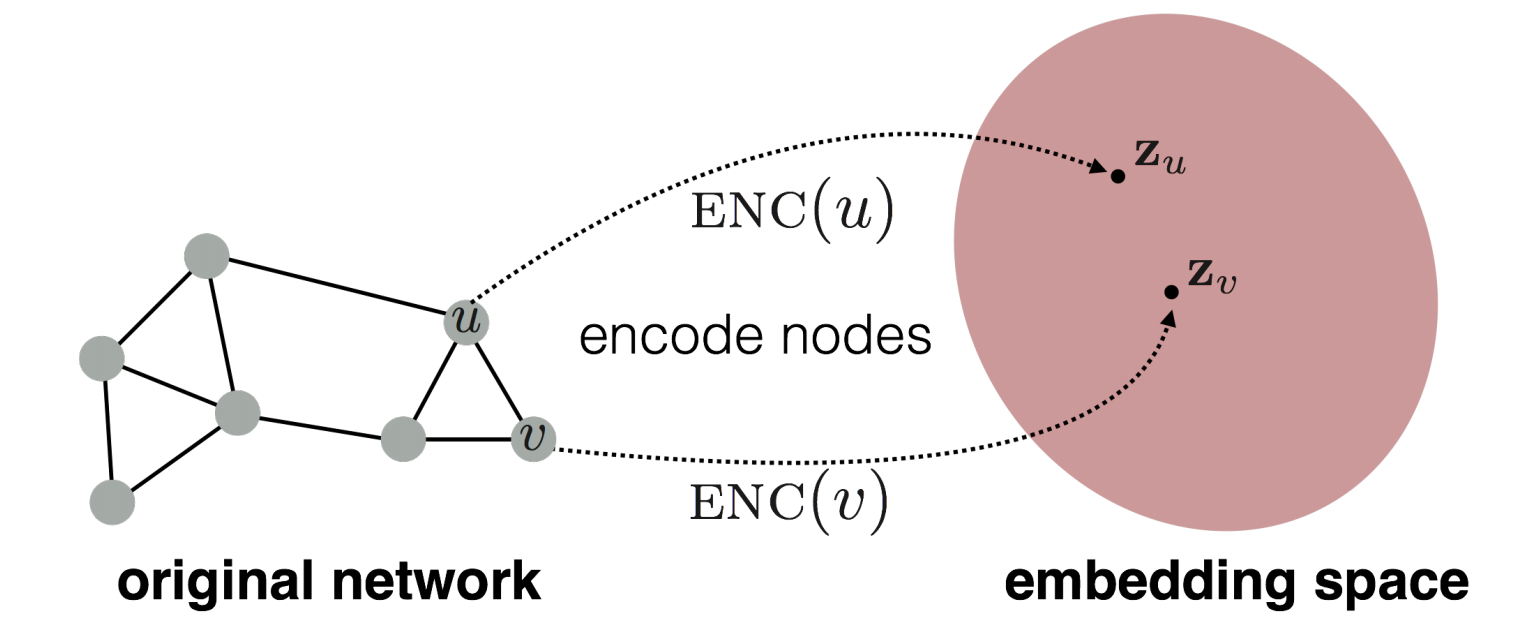
\includegraphics[width=0.8\textwidth]{embedding.png}
		\caption{Network Embedding}
		\cite{leskovec2021lecture}
		\label{fig:embedding}
	\end{figure}

	\noindent To generate node embeddings of a graph, one has to define an
	encoder which transforms nodes in a graph into their embedding space as
	shown in figure \ref{fig:embedding}. The nodes must be embedded in such a
	manner that similar nodes in the graph are also embedded closely in the 
	embedding space. A common measure for similarity is to find vector embeddings 
	$z$ of nodes $u$ and $v$ such that \citep{leskovec2021lecture}:

	\begin{equation}
		z_u^Tz_v \approx similarity(u,v)
		\label{eq:dot_sim}
	\end{equation}

	\noindent The dot product of the two node embedding vectors shown in
	equation \ref{eq:dot_sim} should thus approximately equal the similarity of 
	the corresponding nodes in the graph. There are different approaches for 
	defining node similarity. Graph factorization was introduced as an early 
	solution \citep{ahmed2013distributed}. More recent and successful approaches 
	include methods which make use of random walks. In the context of random 
	walks, similarity is defined as \citep{leskovec2021lecture}:

	\begin{equation}
		z_u^Tz_v \approx \text{Probability that node $u$ and $v$
								co-occur on a random walk over the graph}
	\label{eq:random_similartiy}
	\end{equation}

	\noindent The models DeepWalk \citep{perozzi2014deepwalk} and its 
	generalization Node2Vec \citep{grover2016node2vec} successfully apply the
	similarity measure shown in equation \ref{eq:random_similartiy}. Another 
	noteworthy model called LINE \citep{tang2015line} also makes use of random
	walk co-occurrences as its similarity measure. In order to remain focused,
	only DeepWalk and Node2Vec are considered for this thesis. These two models
	are well suited for the given task and are among the most popular graph
	representation learning methods. \\

	\noindent DeepWalk and Node2Vec make use of methods which have its origin in 
	natural language processing (NLP). Specifically they makes use of the 
	Skip-Gram model introduced by \cite{mikolov2013efficient,mikolov2013distributed}. 
	The Skip-Gram model is a core component of DeepWalk and Node2Vec, which is why 
	it is explained in detail before proceeding to DeepWalk and Node2Vec. \\

	\noindent In NLP words are one-hot encoded as inputs for the Skip-Gram model 
	which learns vector representations of the input words. The aim of the
	Skip-Gram model is then to predict the context of the input word by
	predicting the neighboring words in a sentence. A basic overview of the 
	Skip-Gram model is provided in figure \ref{fig:skip_gram}. 

	\begin{figure}[h]
		\centering
		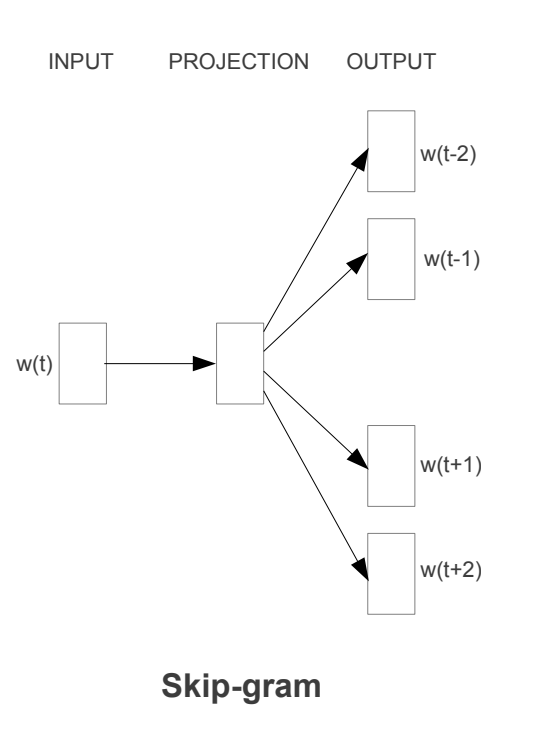
\includegraphics[width=0.4\textwidth]{skip_gram.png}
		\caption{Skip-Gram Architecture}
		\cite[p. 5]{mikolov2013efficient}
		\label{fig:skip_gram}
	\end{figure}

	\noindent The basic layout shown in figure \ref{fig:skip_gram} depicts the
	high-level procedure of the Skip-Gram model. To make this model more
	specific, the input corresponds to the one-hot encoded vector at row $t$ of
	the input matrix $W$ with dimensions $T \times T$, where every row 
	corresponds to a one-hot encoded word. $W(t)$ is linearly passed to the
	projection, which involves calculating the dot product of $W(t)$ with the 
	weight matrix $\Phi$ which has dimensions $T \times D$. $D$ refers to the
	number of dimensions which are to be included in the projection vector $h$ 
	and is a hyper parameter. The projection vector $h$ is then linearly passed
	again with another weight matrix $\Psi$ which has dimensions $D \times T$.
	This creates the output vector $u$ which is then used to predict the correct
	context word $c$ from the vocabulary of $C$ number of context words. To do 
	so, the training target is set to maximize the average $\log$ probability 
	of the correct context word for every input word $w_{t}$. More formally 
	\citep[p. 2]{mikolov2013distributed}:

	\begin{equation}
		\frac{1}{T}\sum_{t=1}^{T}\sum_{-c \leqslant j \leqslant c,j\neq0}\log
		p(w_{t+j}\mid w_{t})
		\label{eq:skip_traintarget}
	\end{equation}

	\noindent To calculate the probability of the context word given the input
	word $w_{t}$, the Softmax function is applied to the output layer $u$ in the 
	manner shown by Mikolov et al. \citeyearpar[p. 3]{mikolov2013distributed}. 
	This calculates a normalized probability for every context word given $w_{t}$. To 
	formalize this in terms of a loss function, the training target shown in 
	equation \ref{eq:skip_traintarget} can be rewritten as follows for every
	input word $w_{t}$:

	\begin{equation}
		\begin{split}
		\mathcal{L} =& - \log p(w_{t-c},\dots,w_{t-1},w_{t+1},\dots,w_{t+c}\mid w_{t})\\
			=& - \log \prod_{c=1}^{C}\frac{\exp(u_{c,j_{c}^{*}})}{\sum_{j'=1}^{T}
			\exp(u_{j'})}\\
			=&	- \sum_{c=1}^{C} u_{j_{c}^{*}} + C \cdot \log
								\sum_{j'=1}^{T} \exp(u_{j'})
		\label{eq:deepwalk_loss}
	\end{split}
	\end{equation}

	\noindent The notation was slightly adjusted, where $u_{j_{c}^{*}}$ refers
	to the index of the output vector $u$ which corresponds to the actual
	context word $c$ given the input word $w_{t}$. In turn, 
	$\sum_{j'=1}^{T}\exp(u_{j'})$ is a summation over all exponentiated output 
	representations $u_{j'}$ of all $T$ number of words given the input word 
	$w_{t}$. The calculated loss is then used to update the trainable model 
	parameters $\Phi$ and $\Psi$ using gradient descent via a backward 
	propagation function analogues to what is used for standard neural 
	networks. The desired output of the Skip-Gram model is the weight matrix
	$\Phi$ which once the model is sufficiently trained, corresponds to the
	vector representation or embeddings of the input words. \\

	\noindent The same principle shown in the Skip-Gram model can be applied
	to graphs in a modified version. First, nodes in a graph can be one-hot
	encoded the same way as words. This means, that nodes can be used as input
	data in a similar fashion as words. Based on this idea, DeepWalk by
	\cite{perozzi2014deepwalk} achieved a big breakthrough for graph
	representation learning. The DeepWalk algorithm builds on top of the 
	Skip-Gram model and uses fixed-length random walks for learning the node 
	embeddings. To provide a better overview of the DeepWalk algorithm, 
	the pseudo-code is presented in algorithm \ref{algo:DeepWalk} \& 
	\ref{algo:SkipGram} \citep[p. 704]{perozzi2014deepwalk}.
	
	\begin{algorithm}[h]
		\scriptsize
		\SetAlgoLined
		\KwIn{graph $G(V,E)$}
		window size $w$\\
		embedding size $d$\\
		walks per vertex $\gamma$\\
		walk length $t$\\
		\KwOut{matrix of vertex representations $\Phi \in \mathbb{R}^{\mid V
		\mid \times d}$}
		\nl Initialization: Sample $\Phi$ from $\mathcal{U}^{\mid V
		\mid \times d}$ \\
		\nl Build a binary Tree $T$ from $V$ \\
		\nl \For{$i=0$ to $\gamma$}{
		\nl		$\mathcal{O}$ = Shuffle($V$) \\
		\nl		\ForEach{$v_i \in \mathcal{O}$}{
		\nl			$\mathcal{W}_{vi} = RandomWalk(G,v_i,t)$\\
		\nl			SkipGram($\Phi,\mathcal{W}_{vi}, w$)
				}
			}
		\caption[DeepWalk]{DeepWalk($G,w,d,\gamma,t$)}
		\label{algo:DeepWalk}
	\end{algorithm}
	
	\begin{algorithm}[h]
		\scriptsize
		\SetAlgoLined
		\nl \ForEach{$v_j \in \mathcal{W}_{vi}$}{
		\nl		\ForEach{$u_k \in \mathcal{W}_{vi}[j-w:j+w]$}{
		\nl			$J(\Phi) = - \log \Pr(u_k \mid \Phi(v_j))$\\
		\nl			$\Phi = \Phi - \alpha * \frac{\partial J}{\partial \Phi}$
				}
			}
		\caption[SkipGram]{SkipGram($\Phi,\mathcal{W}_{vi},w$)}
		\label{algo:SkipGram}
	\end{algorithm}
	
	\vspace{5mm}
	
	\noindent The DeepWalk algorithm shows, that for every node $v\in G$ a
	fixed length random walk is created. Every node on the random walk is used
	as a one-hot encoded input for the Skip-Gram model. The context nodes of the
	input node correspond to the input nodes' neighbors on the random walk 
	within the window size $w$. This procedure is repeated for $\gamma$ 
	number of random walks which in turn concludes one training epoch. The rows
	of $\Phi$ then correspond to the node embeddings where
	$\Phi_{u}=z_{u}^{T}$. Lastly, the dot product of any two node embedding
	vectors, $z_{u}^{T}z_{v}$, approximately equals the probability, that the
	two nodes co-occur on a random walk as outlined in equation 
	\ref{eq:random_similartiy}. Please note, that the DeepWalk algorithm often 
	uses more efficient approximation methods to calculate the loss function
	shown in equation \ref{eq:deepwalk_loss}. These approximation methods
	include hierarchical Softmax which makes use of a binary tree or negative 
	sampling. Both approximation methods are outlined in the paper by 
	\cite{mikolov2013distributed}. \\

	\noindent This is in principle the model which will be used to find the node
	embeddings of a graph. For the application, the Node2Vec algorithm by
	\cite{grover2016node2vec} will be employed, which is a generalization of 
	the DeepWalk algorithm. Node2Vec allows for the deployment of biased random 
	walks. In particular, it allows to set probabilities as to whether the 
	random walk is biased towards breadth-first search (BFS) or depth-first 
	search (DFS). Depending on the network structure, setting an appropriate 
	bias can greatly improve the quality of the embeddings. If no bias towards 
	BFS or DFS is set, an unbiased random walk is employed which is when
	the output of the Node2Vec algorithm corresponds to the output of the 
	DeepWalk algorithm. More precisely, this occurs when the search bias is set
	to $\alpha = 1$ with $p=q=1$ as outlined in the Node2Vec paper 
	\citep[p. 860]{grover2016node2vec}. The results revealed, that an unbiased 
	random walk embedded the nodes very well. For that reason, the Node2Vec 
	algorithm is not explained in further detail as the relevant parts are 
	covered by the simpler and reader friendlier DeepWalk algorithm. If
	interested, the pseudo-code for the Node2Vec algorithm is provided in the 
	article by Grover \& Leskovec (\citeyear[p. 859]{grover2016node2vec}). \\

	\noindent The resulting node embeddings can then be used for downstream
	machine learning tasks using standard methods. An additional benefit of 
	graph representation learning is that the nodes can be encoded into an 
	arbitrary number of dimensions. In this sense, graph representation 
	learning can be used as a powerful dimensionality reduction strategy. 
	The node embeddings correspond to the features used for downstream 
	machine learning tasks. The features were thus learned automatically using 
	the DeepWalk or Node2Vec algorithm. This approach directly takes care of the 
	otherwise at times tedious feature selection process. With this approach, 
	only the number of features need to be defined for feature selection. This 
	is a big advantage and can save a lot of time when working with graphs. 

	\subsection{Graph Neural Networks}
	\label{section:GNN_theory}

	This section provides an overview of the theory for Graph Neural Networks
	(GNN). Within the family of GNNs, there are a myriad of different models 
	available and every few months new models are published. GNNs are currently 
	very popular and benefit from a large research output. This thesis will 
	focus on two popular and established GNN approaches which are:

	\begin{enumerate}
		\item Graph Convolutional Networks
		\item GraphSage
	\end{enumerate}
	
	\noindent Before presenting the two above mentioned methods, a general
	overview of the GNN framework is given. First the required setup is
	defined \citep{leskovec2021lecture}:

	\begin{itemize}
		\setlength\itemsep{0.2em}
		\item $G(V,E)$ is a graph with a set of vertices and edge connections
		\item $V$ is a set of vertices
		\item $A$ is the adjacency matrix of graph $G$
		\item $X \in \mathbb{R}^{\mid V\mid \times F}$ is a matrix containing
			the node features
		\item $v$ is a node $\in V$ and $\mathcal{N}(v)$ is the set of 
			neighbors of node $v$
	\end{itemize}

	\noindent If there are no node features present, $X$ can be defined as a 
	one-hot encoded vector. A naive approach for building a GNN would be to
	append the columns of the adjacency matrix to the feature matrix. This
	combined matrix would then be used as the input for a standard
	artificial neural network. The problem with this approach is, that the 
	input is not order invariant and that the trained model cannot be applied 
	to graphs of different sizes \citep{leskovec2021lecture}. \\

	\noindent Modern GNNs have overcome this problem by drawing inspiration from 
	Convolutional Neural Networks (CNN) and its famous filtering mechanism as 
	outlined by \cite{krizhevsky2012imagenet}. CNNs typically work with grid 
	structured input data such as pixels of images. The convolutional filter 
	then samples the input grid using a filter with a specified size 
	(e.g. $3\times3$ grid filter). Similarly, GNNs sample a graph using the node 
	neighbors $\mathcal{N}(v)$ of node $v$ as a filter. The filter can then be 
	fine tuned in the sense of how many $k$-hops of neighbors to consider 
	(e.g. 1-hop: immediate neighbors of $v$, 2-hop: include neighbors of $v$'s 
	neighbors etc.). In terms of implementation, the number of $k$-hops is set 
	by the number of graph convolutional layers included in the GNN model. An 
	illustration of this mechanism is shown in figure \ref{fig:GNN_structure}. \\

	\begin{figure}[h]
		\centering
		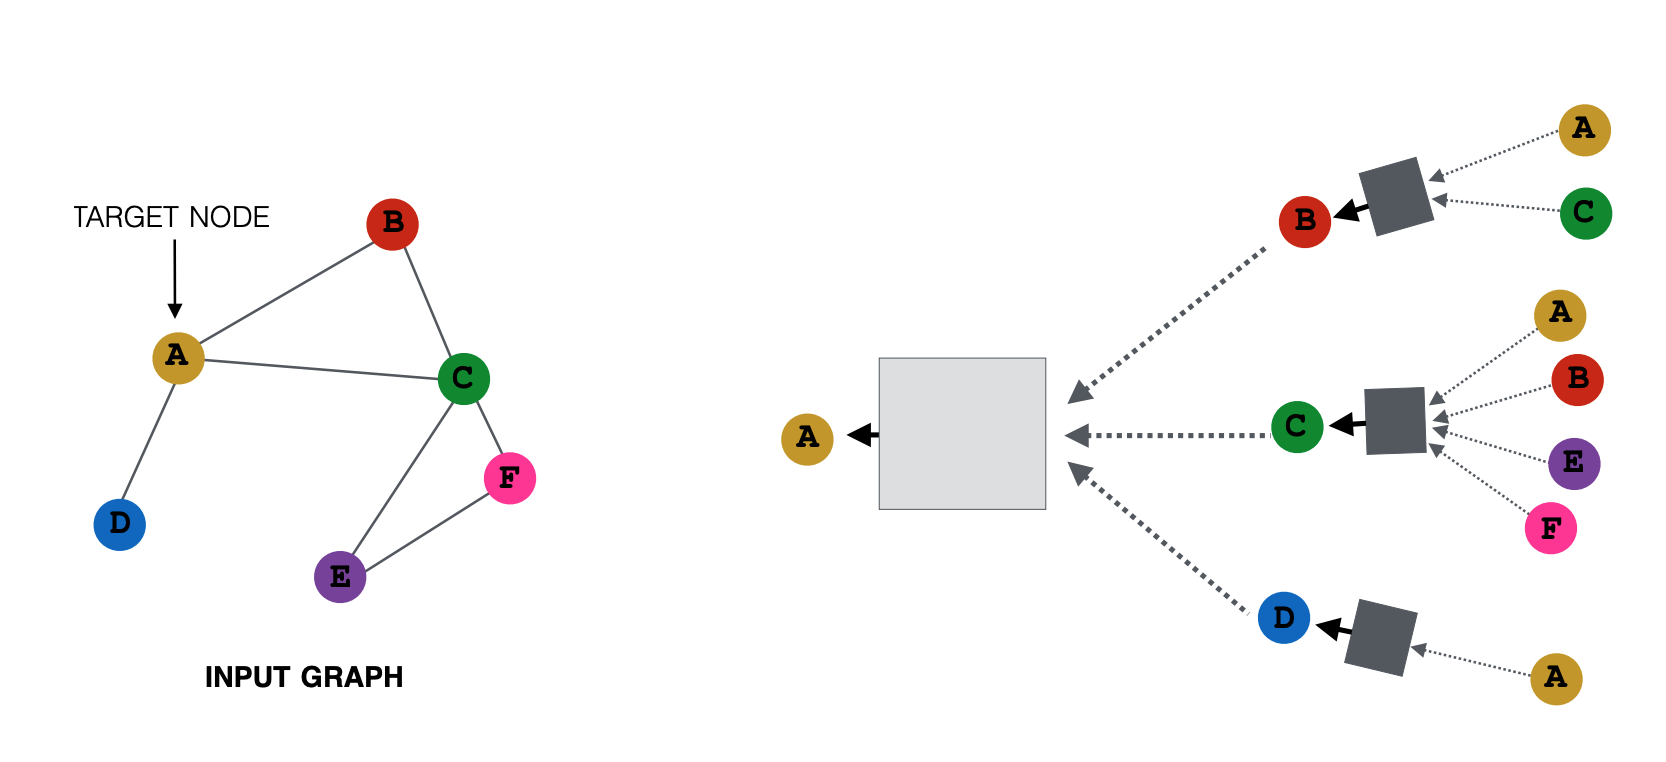
\includegraphics[width=0.8\textwidth]{GNN.png}
		\caption{GNN Structure}
		\cite{leskovec2021lecture}
		\label{fig:GNN_structure}
	\end{figure}

	\noindent The GNN structure outlined in figure \ref{fig:GNN_structure} 
	shows an example of a 2-hop or 2 layer GNN. The 1-hop convolutional layer 
	considers the neighboring nodes of the target node A. The 2-hop layer 
	considers the neighbors of node A's neighbors. Note, that the target node A 
	is included as an input node in the 2-hop layer. This is reasonable as node 
	A itself is also a neighboring node to its neighbors. Taking the example 
	shown in figure \ref{fig:GNN_structure}, the challenge for the GNN is to 
	find node embeddings based on local network neighborhoods \citep{leskovec2021lecture}. 
	The node embeddings at layer 0 correspond to the features of the input nodes 
	where $X = H^{(0)}$. A typical procedure for a GNN model is outlined in 
	algorithm \ref{algo:GNN_struct} 
	\citep{hamilton2017inductive,leskovec2021lecture,you2020design}.	

	\begin{algorithm}[h]
		\scriptsize
		\SetAlgoLined
		\KwIn{Graph $G(V,E)$;}
		\myinput{input features $\{x_v,\forall v \in V\}$;}
		\myinput{node labels $\{y_v, \forall v \in V\}$;}
		\myinput{depth/layers $K$}
		\myinput{Trainable and layer specific parameters $\Theta^{k}$ where
		$W^{k}\in\Theta^{k}, \forall k \in
					\{1,\dots,K\}$;}
		\myinput{non-linearity $\sigma$;}
		\myinput{differentiable aggregator functions $AGGREGATE_{k},\forall k \in
					\{1,\dots,K\}$;}
		\myinput{neighborhood function $\mathcal{N}_{k}:v\rightarrow 2^{V},\forall k \in
					\{1,\dots,K\}$;}
		\myinput{loss function $\mathcal{L}$ such as cross entropy $CE$;}
		\myinput{learning rate $\alpha$}
		\KwOut{Vector representations $z_v, \forall v\in V$}
		\nl Initialize parameters $\Theta$ from $\mathcal{U}$\;
		\nl $h_{v}^{0} = x_{v},\forall v \in V$\\
		\nl \For{Number of epochs}{
		\nl \For{$k=1\dots K$}{
		\nl		\ForAll{$v\in V$}{
		\nl			$h_{\mathcal{N}(v)}^{k} \leftarrow AGGREGATE_k\left(
					{h_{u}^{k-1},\forall u \in\mathcal{N}_{k}(v)}\right)$\;
		\nl			$h_{v}^{k} \leftarrow\sigma \left(W^{k}\cdot 
							CONCAT(h_{v}^{k-1},h_{\mathcal{N}(v)}^{k})\right)$\;
					}		
		\nl		$h_{v}^{k} \leftarrow h_{v}^{k}/\lVert h_{v}^{k}\rVert_{2}$	
   			}
		\nl $z_v = h_{v}^{K},\forall v \in V$\;
		\nl $\mathcal{L}(\Theta)=\sum_{v=1}^{\mid V \mid} CE(y_{v},z_{v})$\;
		\nl $\Theta = \Theta - \alpha\cdot\frac{\partial\mathcal{L}}{\partial\Theta}$
		}
		\caption{Typical GNN Algorithm for Model Training}
		\label{algo:GNN_struct}
	\end{algorithm}

	\noindent Algorithm \ref{algo:GNN_struct} is not meant to be considered as
	a complete overview and should be rather regarded as an example of a typical 
	GNN structure. In addition, one should split the data into training-
	and validation sets to ensure a good model fit. GNNs are flexible in that a 
	myriad of modifications can be added to the GNN layers similar to the 
	possibilities of CNNs or ANNs. The defining features of different GNN 
	methods usually involve the selection of different message passing methods 
	and aggregation strategies. An excellent overview regarding the design space 
	for GNNs is provided in the articles by \cite{you2020design} and 
	\cite{zhou2020graph} as a reference. Of course there are exceptions and 
	alternative procedures exist. The GNN methods evaluated in this thesis and 
	most successful GNNs however tend to follow a variation of the structure 
	shown in algorithm \ref{algo:GNN_struct}.  \\

	\noindent In terms of interpretation, the output of the first GNN layers in
	figure \ref{fig:GNN_structure} (gray boxes) corresponds to the hidden layer 
	representations of the direct neighbors of the target node A. The output of 
	the final GNN layer corresponds to the node embedding $z_{A}$ of the target 
	node A. This should appear familiar when comparing this approach to the graph 
	representation learning method outlined in the previous section. 
	GNNs can indeed be used for unsupervised learning tasks such as learning 
	node embeddings. Good examples for generating node embeddings are shown in 
	the articles regarding Graph Convolutional Networks by \cite{kipf2016semi} 
	and GraphSage by \cite{hamilton2017inductive}. As shown in algorithm 
	\ref{algo:GNN_struct}, GNNs can directly be applied for machine learning
	tasks such as customer classification. This is where GNNs are especially 
	powerful, and differ to the Graph Representation Learning algorithms 
	outlined in the previous section. GNNs are flexible tools and can be used 
	in various settings such as graph representation learning, clustering, 
	classification and link prediction tasks among others \citep{zhou2020graph}. \\

	\noindent Having introduced the general functionality of GNNs, the methods
	Graph Convolutional Networks and GraphSage are introduced in detail in the
	following two sections. 

	\subsubsection{Graph Convolutional Networks}
	
	\noindent The Graph Convolutional Network (GCN) was introduced by 
	\cite{kipf2016semi} and makes use of simplified spectral graph
	convolutions. The author Thomas Kipf \citeyearpar{kipf2016online} provides 
	excellent explanations on his website which is used as inspiration for
	presenting the theory\footnote{Website Thomas Kipf: 
	\url{https://tkipf.github.io/graph-convolutional-networks/}}. As outlined, 
	GNNs typically differ with regards to the type of message passing and 
	aggregation strategy applied. GCNs make use of the following forward 
	propagation function \citep[p. 2]{kipf2016semi}:

	\begin{equation}
		H^{(l+1)} = \sigma\left(\tilde D^{-\frac{1}{2}}\tilde A \tilde
		D^{-\frac{1}{2}}H^{(l)}W^{(l)}\right)
		\label{eq:GCN}
	\end{equation}
	
	\noindent The variables in equation \ref{eq:GCN} are defined as follows:

	\begin{itemize}
		\setlength\itemsep{0.2em}
		\item $H^{l}\in\mathbb{R}^{N \times D}$ refers to the embedding matrix
			at layer $l$ where $N$ refers to the number of nodes $\mid V \mid$
			and $D$ refers to the number of embedding dimensions. The input
			embedding matrix is set equal to the feature matrix, $H^{(0)}=X$.
		\item $W^{l}$ refers to the trainable and layer specific weight matrix
			for the linear message passing employed in the GCN model.
		\item $\tilde A = A + I_N$, where $A$ is the adjacency matrix of the
			input graph $G$. The identity matrix is added so that self-loops
			are considered. This is necessary as the target node of every layer
			is considered in the aggregation process as previously outlined.
		\item $\tilde D_{ii} = \sum_{j}\tilde A_{ij}$ is a diagonal matrix
			containing the degree distributions of the modified adjacency
			matrix $\tilde A$.
		\item $\sigma(\cdot)$ refers to an activation function such as ReLU or
			Softmax.
	\end{itemize}

	\noindent To provide a better overview, the compact notation shown in 
	equation \ref{eq:GCN} is expanded in the following equation for one GCN
	layer \citep{Dubois2019}:

	\begin{equation}
		h_{ij}^{(l)} = \sigma\left(\sum_{(i,j)\in
		\mathcal{N}(v)}\frac{\tilde a_{ik}h_{kj}^{(l-1)}}{\sqrt{\tilde
d_{k,k}\tilde d_{i,i}}} W^{(l)}\right)
		\label{eq:GCN_expand}
	\end{equation}
	
	\noindent In Equation \ref{eq:GCN_expand} $h_{ij}^{(l)}$ refers to the 
	hidden layer representation of node $i$ at layer $l$ considering the set of
	neighbors $j$. $h_{kj}^{(l-1)}$ corresponds to the hidden layer
	representation of node $k$ at layer $l-1$ which is part of the set of 
	neighbors $j$. In terms of filtering strategy, $(i,j) \in \mathcal{N}(v)$. 
	This means that both set of nodes $i$ and $j$ are neighbors of the target 
	node $v$ at layers $l$ and $(l-1)$ respectively. Linear message
	passing is then performed for every neighbor in $j$ at layer $l-1$. The node 
	in the graph $G$ at position $\tilde a_{ik}$ of the modified adjacency matrix 
	selects the nodes for which a connection between $h_{ij}^{(l)}$ and
	$h_{kj}^{(l-1)}$ exists. The embeddings $h_{kj}^{(l-1)}$ of the selected 
	nodes are normalized by the symmetric degree distributions of the previous 
	hidden layer node $\tilde d_{k,k}$ and the new hidden layer node $\tilde d_{i,i}$.
	Afterwards the normalized embeddings are message passed by multiplying it
	with the shared weight matrix $W^{(l)}$. Lastly, the sum of the received
	messages is taken in terms of aggregation strategy and the resulting
	aggregate is passed through the activation function to yield $h_{ij}^{(l)}$.
	Note, that the aggregation strategy involves taking a weighted sum thanks
	to the symmetric normalization. \\

	\noindent The detailed explanations given above show the procedure for
	one layer of a GCN. Returning now to compact notation, this procedure can be
	expanded for two or more GCN layers. First, the notation is further
	simplified by defining $\hat A = \tilde D^{-\frac{1}{2}}\tilde A \tilde
	D^{-\frac{1}{2}}$. An example of a two-layer GCN is then given as follows 
	where $Z$ refers to the embedding or output of the target node 
	\citep[p. 3]{kipf2016semi}:

	\begin{equation}
		Z = f(X,A) = \text{softmax}\left(\hat A \;\text{ReLU}\left(\hat A X
		W^{(0)}\right)W^{(1)}\right)
	\label{eq:GCN_forward}
	\end{equation}

	\noindent Finally, the model parameters are updated analogues to the
	procedure outlined in algorithm \ref{algo:GNN_struct}. The main distinctive
	feature for the GCN is the differing forward propagation function. 

	\subsubsection{GraphSage}
	
	\noindent This section introduces GraphSage by \cite{hamilton2017inductive} 
	which can be thought of as the inductive counterpart of the GCN presented 
	in the previous section. Inductive refers to the capability of not only 
	performing machine learning tasks on the graph used for training but to 
	apply the trained GNN model to new and unseen graphs. This is a large leap 
	as GCN for instance can only be used to predict unseen nodes on the graph 
	which was used for training. This is very limiting for the application of 
	GNNs in a practical setting. GraphSage achieves this by applying different 
	aggregation strategies and sampling the neighborhood $\mathcal{N}(v)$.
	Specifically, the GraphSage model only considers a fixed number of 
	uniformly random sampled neighbors from $\mathcal{N}(v)$ with depth $K$. A 
	graphical example of this procedure is shown in figure \ref{fig:GraphSage_sample}:

	\begin{figure}[h]
		\centering
		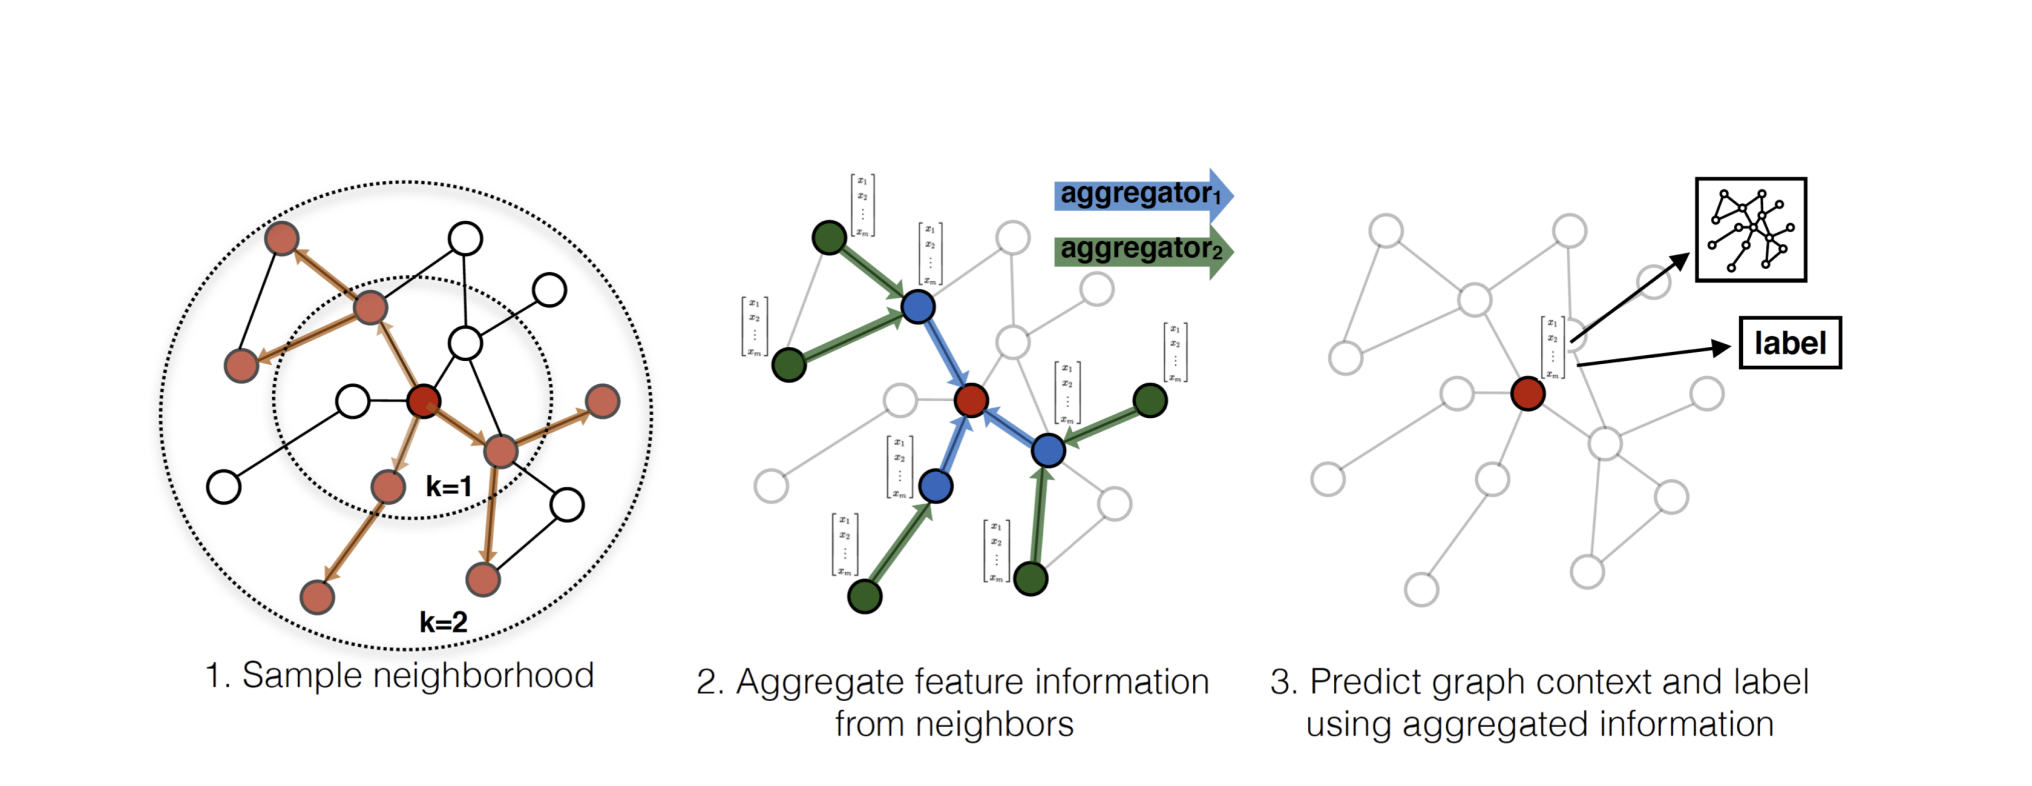
\includegraphics[width=0.8\textwidth]{graphsage.png}
		\caption{GraphSage Sampling}
		\cite[p. 2]{hamilton2017inductive}
		\label{fig:GraphSage_sample}
	\end{figure}

	\noindent The steps shown in figure \ref{fig:GraphSage_sample} are similar
	to the procedures for GCNs. The pseudo code for the GraphSage forward 
	propagation function is given in algorithm \ref{algo:GraphSage} 
	\cite[p. 12]{hamilton2017inductive}. \\


	\begin{algorithm}[h]
		\scriptsize
		\SetAlgoLined
		\KwIn{Graph $G(V,E)$;}
		\myinput{input features \{$x_v,\forall v \in \mathcal{B}$\};}
		\myinput{depth $K$;} 
		\myinput{weight matrices $W^{k},\forall k \in\{1,\dots,K\}$;}
		\myinput{non-linearity $\sigma$;}
		\myinput{differentiable aggregator functions $AGGREGATE_k,\forall k \in
					\{1,\dots,K\}$;}
		\myinput{neighborhood sampling functions, $\mathcal{N}_k:v\rightarrow
					2^{v},\forall k \in \{1,\dots,K\}$}
		\KwOut{Vector representations $z_v$ for all $v\in\mathcal{B}$}
		\nl $\mathcal{B}^{K}\in\mathcal{B}$\\
		\nl \For{$k=K\dots 1$}{
		\nl		$\mathcal{B}^{k-1}\leftarrow\mathcal{B}^{k}$\\
		\nl		\For{$u\in\mathcal{B}^{k}$}{
		\nl			$\mathcal{B}^{k-1}\leftarrow\mathcal{B}^{k-1}\cup\mathcal{N}_{k}(u)$
					}
				}
		\nl $h_{u}^{0}\leftarrow x_{v},\forall v \in \mathcal{B}^{0}$\\
		\nl \For{$k=1\dots K$}{
		\nl		\For{$u\in\mathcal{B}^{k}$}{
		\nl			$h_{\mathcal{N}(u)}^{k}\leftarrow
					AGGREGATE_k(\{h_{u'}^{k-1},\forall u'\in \mathcal{N}_{k}(u)\})$\;
		\nl			$h_{u}^{k}\leftarrow\sigma\left(W^{k}\cdot
					CONCAT(h_{u}^{k-1},h_{\mathcal{N}(u)}^{k})\right)$\;
		\nl			$h_{u}^{k} \leftarrow h_{u}^{k}/\lVert
					h_{u}^{k}\rVert_{2}$		
				}		
			}
		\nl $z_v \leftarrow h_{u}^{K},\forall u \in \mathcal{B}$
		\caption{GraphSAGE Minibatch Forward Propagation Algorithm}
		\label{algo:GraphSage}
	\end{algorithm}
	
	\noindent Note that algorithm \ref{algo:GraphSage} assumes that the
	parameters of the aggregator functions and the weight matrices $W$
	are known. Algorithm \ref{algo:GraphSage} thus shows the forward
	propagation of a trained GraphSage model. The model is trained by
	optimizing the model parameters using mini-batch training for a specified 
	number of epochs. The training procedure can be implemented by using an
	adaptation of the general procedure shown in algorithm \ref{algo:GNN_struct}. 
	Note, that the parameters of the aggregation functions and the weight 
	matrices $W$ are all layer specific elements of $\Theta$ in algorithm 
	\ref{algo:GNN_struct}. For algorithm \ref{algo:GraphSage}, $\mathcal{B}$ 
	refers to the mini-batches of vertices taken from the set of vertices $V$ 
	of the graph $G(V,E)$. \\
	\newpage
	\noindent There are three aggregator types proposed for GraphSage
	\citep{hamilton2017inductive}:

	\begin{enumerate}
		\setlength\itemsep{0.2em}
		\item Mean aggregation
		\item Max pooling
		\item LSTM (long short-term memory) aggregation
	\end{enumerate}

	\noindent The three proposed aggregation strategies are briefly introduced
	as follows:

	\paragraph{Mean Aggregation} \mbox{}\\
	\noindent This type of aggregation is similar to the GCN and takes the
	average of the received messages from the message passing procedure. The 
	difference to GCN is that mean aggregation does not rely on the full graph 
	Laplacian and makes use of a slightly different normalization approach. The 
	aggregation process differs to the one shown in algorithm 
	\ref{algo:GraphSage} and replaces the procedures in line 9 and 10 with 
	\citep[p. 5]{hamilton2017inductive}:

	\begin{equation}
		h_{v}^{k} \leftarrow \sigma\left(W\cdot
		\text{MEAN}(\{h_{v}^{k-1}\}\cup\{h_{u}^{k-1},\forall u \in \mathcal{N}(v)\})\right)
	\end{equation}

	\paragraph{Max-Pooling Aggregation} \mbox{}\\
	\noindent Max-Pooling aggregation refers to the application of an 
	element-wise $\max$ operator. This means 
	that of the neighbors, only the largest element-wise features are considered. 
	More formally, max-pooling aggregation is defined as follows and is used 
	for the aggregation shown in line 9 of algorithm \ref{algo:GraphSage} 
	\citep[p. 6]{hamilton2017inductive}:

	\begin{equation}
		AGGREGATE_{k}^{pool} = \max\left(\sigma(\{W_{pool}h_{u_{i}}^{k} +
		b),\forall u_{i} \in \mathcal{N}(v)\}\right)
	\end{equation}

	\noindent Note, that $W_{pool}$ refers to a separate weight matrix for the
	one layer message passing of the max-pooling aggregation. In principle, an 
	arbitrary number of layers could be added for max-pooling. The authors 
	\cite{hamilton2017inductive} however focus on the case with one layer. The
	parameters of max-pooling are learned analogues to the other GraphSage
	model parameters. \\ 

	\paragraph{LSTM Aggregation} \mbox{}\\
	\noindent LSTM is the last aggregation strategy proposed for GraphSage and
	uses the LSTM recurrent neural network (RNN) first introduced by
	\cite{hochreiter1997long} as an aggregation strategy. LSTMs are not
	permutation invariant which is a requirement for the aggregation strategy.
	The authors propose using a random permutation of the set of node neighbors 
	to counter this problem \citep[p. 5]{hamilton2017inductive}. The LSTM
	parameters are trained along with the other GraphSage model parameters.  

	\section{Graph Generation}
	\label{section:theory_graphgen} 

	This section introduces the Multiplicative Attribute Graph (MAG) model by
	\cite{kim2012multiplicative}. This model is used to generate
	semi-synthetic graphs from feature data as mentioned in the introduction. 
	Originally, the MAG model was introduced for the purpose of generating 
	realistic graphs from feature data and to show that the resulting graph can 
	obey properties of real-world networks. To show this, Kim \& Leskovec 
	generated random feature data for which the model parameters were set in 
	such a manner, that the resulting graph adheres to a set of real network 
	properties. These network properties include the emergence of a giant
	connected component and a power-law or $\log$-normal degree distribution
	among others \citep[p. 113]{kim2012multiplicative}. While, the creation of a 
	graph which follows real-world network properties would be desirable, it is 
	not the primary target for this thesis. The main goal of the semi-synthetic 
	graph generation is to create a graph that provides useful additional 
	information, which can be exploited using graph machine learning. The MAG 
	model is flexible in this sense, that it can create graphs which are not 
	constrained to adhere to a specific set of network properties. Lastly, 
	\citeauthor{kim2012multiplicative} 
	\citeyearpar[p. 138-139]{kim2012multiplicative} present model parameters 
	which generate graphs that follow real-world network properties. These model 
	parameters can however not be adopted for the task at hand. The parameters 
	were created for a somewhat simpler task which "only" involved randomly 
	generated feature data. These randomly generate features do not correspond
	to any specific features. For that reason, the model parameters can be
	chosen freely such that the generated network follows real world network
	properties. The aim of \citeauthor{kim2012multiplicative} was primarily to
	create random graphs that can adhere to said network properties. For this
	thesis, the same MAG model will applied using real feature data. This makes
	the task of defining the model parameters more difficult as they cannot be
	freely assigned. In addition, the generated graph will be used for machine
	learning which is not an application the authors had considered. In this 
	regard the reason and aim for using the MAG model differs for this thesis 
	compared to the original paper. \\

	\noindent The starting point of the MAG model is a matrix of feature data, 
	$X^{N \times F}$, where $N$ refers to the number of observations 
	and $F$ to the number of features. \citeauthor{kim2012multiplicative} refer 
	to feature data as attributes and they use the terms interchangeably. For this 
	thesis a distinction is made, where features correspond to the full set of 
	feature data and attributes refer to the $K$ number of features used for 
	generating the graph, $G(V,E)$. The attribute data, 
	$B^{N \times K} \subseteq X^{N \times F}$, is therefore a subset of the 
	feature data. As a selection criterion, attribute data must be of such a 
	manner that reasonable link-affinity matrices, $\Theta_{i}$, can be 
	defined. In addition, attribute data must be discrete. For practical
	reasons, the cardinality of the attributes should not be too large.
	Attributes such as age might have to be discretized into 4 or 5 discrete
	age categories. The link-affinity matrix, $\Theta_{i}$, is a matrix
	containing probabilities which are used to estimate the probability of two 
	observations in the dataset $(u,v)$ to form a connection. More specifically, 
	the probability for a connection is calculated given the attributes $a_i$ of 
	observation $u$ and $v$ where $(a_{i}(u),a_{i}(v))\in B$. For example, a 
	reasonable assumption could be to assume, that people which are of the same 
	age group, are more likely to be similar and thus form a connection 
	compared to people which are not of the same age group. Another example for 
	this could be gender in terms of biological sex which is a classical binary 
	setting for a link-affinity matrix. Examples of binary attribute 
	link-affinity matrices $\Theta_i$ are given in 
	figure \ref{fig:link-affinity}.

	\begin{figure}[h]
		\centering
		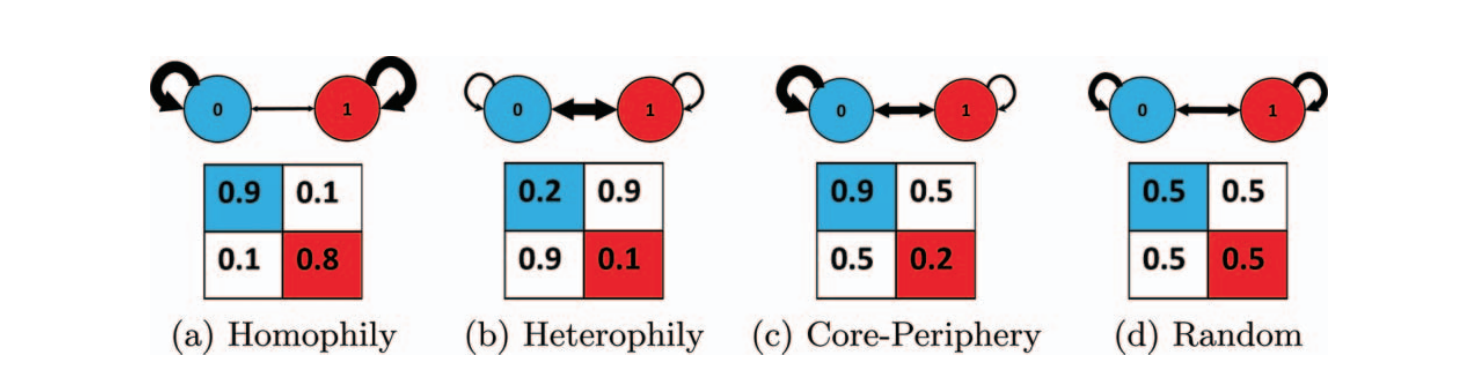
\includegraphics[width=0.9\textwidth]{affinity_matrices.png}
		\caption{Attribute Link-Affinities}
		\cite[p. 118]{kim2012multiplicative}
		\label{fig:link-affinity}
	\end{figure}

	\noindent Figure \ref{fig:link-affinity} shows 4 types of link-affinity
	matrices depending on the type of relationship one wants to model. Homophily 
	refers to love of the same which would make a connection between two
	observations more likely if they have the same attributes. Similarly,
	Heterophily refers to the love of the different where observations which do 
	not have the same attributes are more likely form a connection. 
	Core-periphery is a special case which can be used to generate realistic 
	social-networks in terms of network properties 
	\citep[p. 139]{kim2012multiplicative}. As an example, an attribute could
	indicate whether a person is a member of the local football club. In a
	core-periphery setting, members of the local football club are very likely
	to be connected, while non-members have a significantly lower probability
	of forming a connection. Lastly, random graphs can be generated by setting the
	link-affinity probabilities to 0.5. Given the type of attributes available
	in the data sets, graphs will be generated using homophily structures. The 
	attribute link-affinity matrices, $\Theta_i$, are defined for every attribute 
	and can be set for an arbitrary size of categories within an attribute. 
	More formally for each observation $u \in B$ with $K$ categorical attributes 
	of cardinality $d_i$ for $i = 1,2,\dots,K$ and corresponding link-affinity 
	matrices $\Theta_{i}^{d_{i} \times d_{i}}$ for $i=1,2,\dots,K$, the probability 
	$P[u,v]$ of a connection between observations $(u,v)$ is defined as 
	\citep[p. 119]{kim2012multiplicative}:

	\begin{equation}
		P[u,v] = \prod_{i=1}^{K}\Theta_{i}\left[a_{i}(u),a_i(v)\right]
		\label{eq:MAG}
	\end{equation}

	\noindent In equation \ref{eq:MAG}, $a_{i}(u)$ refers to the value of the 
	$i$th attribute of observation $u$. A schematic representation of the 
	procedure for a binary link-affinity matrix is shown in figure \ref{fig:MAG}.

	\begin{figure}[h]
		\centering
		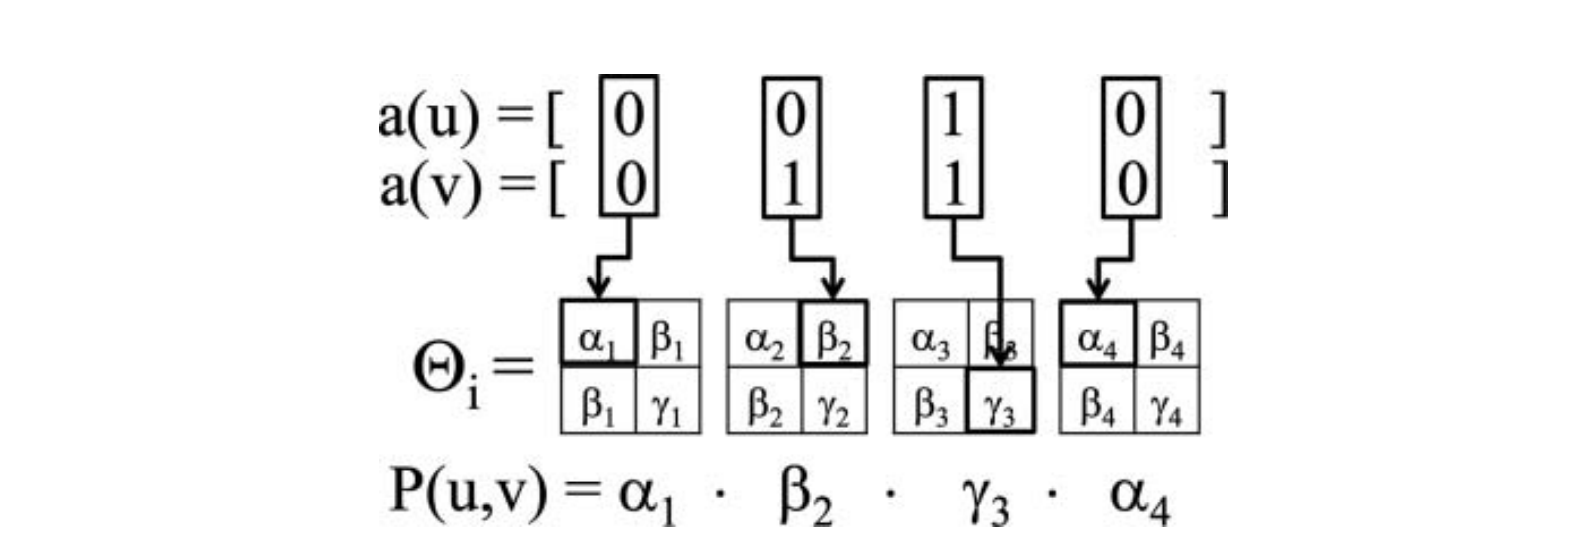
\includegraphics[width=0.8\textwidth]{MAG.png}
		\caption{Schematic Representation of the 
			Multiplicative Attribute Graphs (MAG) Model}
		\cite[p. 120]{kim2012multiplicative}
		\label{fig:MAG}
	\end{figure}
	
	\begin{algorithm}[h]
		\scriptsize
		\SetAlgoLined
		\KwIn{graph node-attribute generation matrix $B^{N \times K}$, where 
			$B\subseteq X^{N \times F}$;}
		\myinput{node attribute vector $a_i$ with
			cardinalities $d_i$ for $i=1,2,\dots,K$;}
		\myinput{link affinity matrices $\Theta_{i}^{d_i \times d_i}$, for $i= 1,2,\dots,K$;}
		\KwOut{adjacency Matrix $A^{N\times N}$ for Graph $G(V,E)$} 
		\nl $B^{K \times N} = B^{T}$ \\
		\nl \For{$j = 1,2,\dots,N$}{
		\nl	$u = B[:,j]$\\
		\nl		\For{$k = 1,2,\dots,N$}{
		\nl			$v = B[:,k]$\\
		\nl			\For{$i = 1,2,\dots,K$}{
		\nl				$P_{j,k} = \prod_{i=1}^{K}\Theta_{i}[a_{i}(u),a_i(v)]$
						}
				}
			}
		\nl $U^{N \times N} = uppertriangular(P)$ with $diag(U)=0$\\
		\nl \For{$i=1,2,\dots,N$}{
		\nl		\For{$j=1,2,\dots,N$}{
		\nl			\If{$U_{i,j} > \mathcal{U}(0,1)$}{
		\nl				$\hat A_{i,j} = 1$} 
		\nl			\Else{$\hat A_{i,j} = 0$}
				}
			}
		\nl $A = \hat A + \hat A^{T}$
		\caption{Multiplicative Attribute Graph Model}
		\label{algo:MAG}
	\end{algorithm}

	\noindent The pseudo-code of the MAG model is depicted in algorithm 
	\ref{algo:MAG} and generates the adjacency matrix $A$ which is then used 
	for constructing the graph $G(V,E)$. The observations of the feature data 
	$X$ which contains the attributes are used as inputs and correspond to the 
	nodes in the resulting graph. More precisely, the order of the generated 
	adjacency matrix $A$, corresponds to the ordering of the feature matrix $X$. 
	Therefore the features can be assigned to the nodes of the generated graph. 
	The procedure outlined in algorithm \ref{algo:MAG} can be summarized with 
	the following sequential steps:

	\begin{enumerate}
		\item Calculate the connection probabilities $P$ between every 
			observation in the attribute matrix $B$ using equation \ref{eq:MAG}. 
		\item As we only work with undirected graphs, the upper triangular
			matrix $U$ of $P$ is taken where the $diag(U) = 0$. The diagonal of
			$U$ is set to 0 to exclude self-loops.
		\item For every element in $U$, draw a random number form a standard
			uniform distribution $\mathcal{U}(0,1)$. If the connection
			probability $P_{u,v}>\mathcal{U}(0,1)$, a 1 in the
			preliminary adjacency matrix $\hat A_{u,v}$ is recorded.
			Otherwise a 0 is recorded.
		\item The preliminary adjacency matrix $\hat A$ is an upper triangular
			matrix with $diag(\hat A) = 0$ and all elements in the lower
			triangular also being equal to 0. As the target is to create an
			undirected graph, the corresponding adjacency matrix is symmetric
			which is why the final adjacency matrix can be created using 
			$A = \hat A + \hat A^{T}$. 
	\end{enumerate}

	\noindent This concludes the required theoretical background for this
	thesis. 

  \label{section:theory}
 

  % Data
    
  This section introduces the datasets used for this thesis. Several approaches
  and datasets were considered for evaluating the success of graph machine
  learning on semi-synthetic graphs. In particular, three datasets were 
  considered with varying degrees of success which are:

  \begin{enumerate}
    \item Self launched survey
    \item Bank telemarketing dataset
    \item US Airline passenger satisfaction survey
  \end{enumerate}

  \noindent The datasets are introduced to the extent that they were successful 
  or useful within the framework of this thesis. In particular, the self 
  launched survey and the bank telemarketing dataset showed to be problematic 
  for different reasons. They however provide valuable insights as
  to when graph machine learning can be successful. These two datasets are 
  therefore only briefly introduced with the focus lying on providing the
  insights gained from these "failed" datasets. The detailed introduction and
  analysis of these datasets is skipped and is deferred to the appendix. The
  airline passenger satisfaction dataset will be presented in detail, as good
  results were achieved using graph machine learning. This dataset will also be
  used for comparing graph machine learning to the standard machine learning
  methods. \\

  \noindent Before introducing the datasets, the programming language and the
   packages used for the analysis are thankfully referenced in the following 
   section.

  \section{Software \& Code}

  The entire thesis was evaluated using the Python 3.8.10 programming
  language \citep{vanRossum2009}. In addition, following open-source python
  packages were thankfully used which are Numpy 1.20.2 \citep{harris2020array},
  Matplotlib 3.3.4 \citep{Hunter2007}, NetworkX 2.5.1 \citep{hagberg2008exploring}, 
  Seaborn 0.11.1 \citep{Waskom2021}, Pandas 1.2.5 \citep{mckinney2010data}, 
  Statsmodels 0.12.2 \citep{seabold2010statsmodels}, Scikit-Learn 0.24.2 
  \citep{pedregosa2011scikit}, Tensorflow 2.4.0 \citep{abadi2016tensorflow}, 
  Pytorch 1.7.0 \citep{paszke2019pytorch}, deep graph library (dgl) 0.6.1 
  \citep{wang2019deep}, tqdm 4.61.1 \citep{da2021tqdm} and Node2Vec 0.4.3 
  \citep{Cohen2021}. \\

  \noindent The data sets as well as the Python code used for creating and 
  analyzing the data can be found in a public GitHub repository\footnote{GitHub
  repository: \url{https://github.com/MichaelvonSiebenthal/MasterThesis.git}}. 
  The Github repository also includes the Python code for the results shown in
  chapter \ref{section:results}. In general any data, analysis and results
  referenced or presented as part of this master thesis can be found in the
  GitHub repository. This is meant to be a general reference to the data and
  Python code used for this thesis and will not be referenced individually for
  every analysis or result presented. The GitHub repository includes a read me
  file which describes what information can be found in which folder and
  document. In addition, the Python Code is written in Jupyter Notebooks which
  allows for detailed descriptions of the used codes using markdown. The GitHub
  repository can thus be considered as a form of appendix for this thesis.

  \section{Self Launched Survey}
  \label{section:self_survey} 

  Initially, the aim was to make use of a self-launched survey which focused on
  a bank client classification task. The classification task was two-fold in 
  that a simpler task focused on classifying bank clients as to whether they 
  would be interested in investing or not. The second classification task
  involved classifying clients according to their investment preferences in
  terms of products (single securities like stocks or bonds, funds, ETFs,
  unsure). The variables used for the graph creation using the MAG model
  included mostly demographic data. Additional data was collected by assessing
  the financial knowledge and behavioral profile of the survey participants by 
  using questions from the financial literacy report of the OECD
  (\citeyear{OECD2017}). The idea was, that demographic data coupled with the 
  financial literacy questions should be provide a suitable database for the bank 
  client classification task. This hypothesis was based on the professional 
  experience of the author of this thesis having worked for over 10 years as a 
  client adviser for a large Swiss bank. \\

  \noindent Unfortunately, only $n=113$ people participated in the survey which 
  in general is very small for a machine learning task.
  Further, the graphs generated using the MAG method were not stable. Due to
  the stochastic element present in the MAG model, the resulting graphs could
  differ dramatically. This lead to significant performance differences for the
  different machine learning methods applied to the resulting graphs.
  Classification accuracies ranged between accuracies of 40 - 95 \%. A remedy
  for this problem could be to assign a fixed probability threshold such as 0.5
  in the MAG model. Using a fixed threshold probability, the MAG model would 
  generate deterministic graphs, which are always the same. The downside however 
  is, that this makes the graph generation process less realistic. In a
  homophily setting this would assume that a connection is formed with any node 
  where $P[u,v]>0.5$. It is unclear without testing, what impact this would
  have on the graph generation and whether it is positive or negative. It is
  well understood, that people often form connections with people that appear
  unlikely from a probabilistic perspective. This consideration would warrant
  the generation of stochastic graphs. The main priority is however to create
  graphs which provide additional information that can be exploited via graph
  machine learning. Having this objective in mind, it warrants further
  investigation for which the results will be presented in section 
  \ref{section:stoch_det}. \\

  \noindent The self-launched survey could not be used for any meaningful
  analysis due to the small sample size. Nevertheless, it provided an
  interesting follow-up question regarding the question of generating
  stochastic- versus deterministic graphs. The dataset was discarded for
  further analysis and the survey data as well as the performed analyses can be
  found in the appendix. 

  \section{Bank Telemarketing Dataset}
  \label{section:bank_data}

  The bank telemarketing dataset first introduced by 
  \cite{moro2011using,moro2014data} was considered as a banking related back-up 
  dataset in case that the self made survey did not yield a sufficient number of 
  responses. The bank telemarketing dataset is based on a marketing campaign at 
  a Portuguese bank. The dataset includes demographic data, data regarding the 
  bank client's wealth, contact success during previous campaigns etc. The
  dataset further provides label data which indicates whether a client invested
  in a short-term deposit after having been contacted. The dataset is therefore
  set-up for a binary classification task. The MAG graph generated from the
  bank telemarketing dataset is shown in figure \ref{fig:Moro}.
 
	\begin{figure}[h]
		\centering
		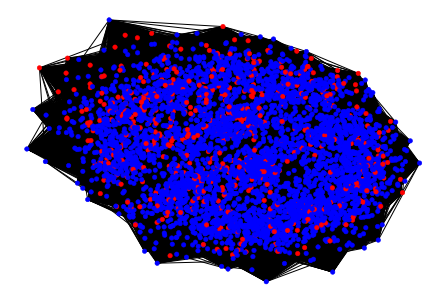
\includegraphics[width=0.7\textwidth]{Moro_network.png}
		\caption{MAG graph of bank telemarketing dataset}
        \label{fig:Moro}
	\end{figure}
  
  \noindent The red dots in figure \ref{fig:Moro} mark the clients which
  decided to invest in the short-term deposit and the blue dots did not invest.
  This figure masks some of the blue nodes due to the figure generation
  process, the general pattern however is apparent. The red nodes are randomly 
  placed in the network which suggests, that graph machine learning will be of
  limited use. The graph further shows, that only a relatively small number of 
  clients appear to have invested in the short-term deposit. To be more precise, 
  only approximately 12\% of bank clients invested in the short-term deposit. 
  The dataset is unbalanced which makes the classification task difficult. Graph 
  representation learning using Node2Vec did not provide any useful results and 
  the GNNs also performed rather poorly. In particular, GNNs tended to classify 
  most clients as non-investors and struggled to accurately classify clients 
  which did invest. Due to the unbalanced data, it is loss optimizing for the
  GNN to predict most nodes as non-investors rather than learning the true
  label. Table \ref{table:Moro_conf} shows the confusion matrix of the 
  classification results for the validation dataset (20\%) using a GraphSage GNN.

  \begin{table}[h]
    \centering
    \begin{tabular}{|l|l|c|c}
      \hline
      \diagbox{\textbf{Label}}{\textbf{Predicted}} & \textbf{Did not invest} &
      \textbf{Invested} \\
      \hline
      \textbf{Did not invest} & 1'026 & 30 \\\hline 
      \textbf{Invested} & 119 & 33 \\
      \hline
    \end{tabular}
    \caption{Confusion Matrix Validation Bank Telemarketing Data}
    \label{table:Moro_conf}
  \end{table}

  \noindent The resulting confusion matrix corresponds to an accuracy of
  approximately 87.67\%. The MAG generation process was repeated multiple times
  for which the GraphSage accuracies ranged between 87 - 90\%. Similar results
  were observed for both graph based methods and standard machine learning 
  methods such as ANNs or support vector machines (SVM). \\

  \noindent Unbalanced datasets are part of a larger and common problem in 
  machine learning. Possible remedies might include using loss functions which 
  penalize false classifications harsher than the standard cross entropy loss 
  function used for the GNNs. Alternatively, one could also reduce the data set 
  by dropping observations such that the remaining dataset is balanced. This 
  approach has its own problems as dropping a large number of observations 
  discards a lot of potentially valuable information. It could also put in 
  question the external validity of the model. These comments point to a 
  separate field of research and could be interesting for a future project. 
  These approaches were not researched in detail and should be taken as 
  suggestions. \\

  \noindent The failure using graph machine learning methods for this dataset
  reveals, that GNNs are not an easy remedy for unbalanced data. Perhaps if the
  network structure provided clusters which corresponded to the labels, GNNs
  could provide superior results. Given the variables available in the dataset
  and the limitations of using the MAG method, this was not possible. In order
  to check, whether network structure could indeed remedy the unbalanced label
  problem, the label of the bank telemarketing dataset was used for the MAG 
  network generation process. The label is normally not included as an
  attribute for the MAG model, as the label data is usually unknown outside of
  the training dataset. The link-affinity probabilities for the label was set
  as follows:

  \[ \Theta_{label} = 
	\begin{pmatrix}
        0.95 & 0.25 \\
		0.25 & 0.95 \\
	\end{pmatrix}
	\] \\
  
  \noindent The resulting MAG graph when considering the label is shown in figure
  \ref{fig:Moro_bias}.

  \begin{figure}[h]
		\centering
		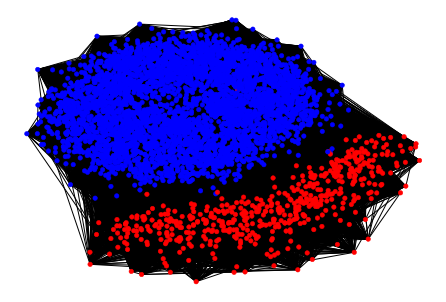
\includegraphics[width=0.7\textwidth]{Moro_network_bias.png}
		\caption{Biased MAG graph of bank telemarketing dataset}
        \label{fig:Moro_bias}
  \end{figure}

  \noindent The nodes shown in figure \ref{fig:Moro_bias} are now nicely
  clustered according to their label. The GNN method GraphSage achieved an 
  accuracy of over 95\% for this graph using otherwise identical feature data
  and model specifications as before. This is of course a form of cheating, as 
  we cannot assume to know the labels of the graph outside of the training 
  setting. In a real-world application, the model would be trained using label
  data and then applied to new data which does not contain the label. We would
  however require the label for the graph generation procedure which makes this
  not a viable approach. Nevertheless, this result shows extremely well when
  graph machine learning can yield superior results compared to standard
  machine learning methods. The key lies in generating a graph with a network
  structure that corresponds to the label. The network structure need not
  necessarily be as clearly separated as shown in figure \ref{fig:Moro_bias}. A
  graph which contains local neighborhood clusters which correspond to the same
  label could yield similar good results. In such a setting, one would have to be
  careful when defining the number of layers, $K$, and neighborhood
  sampling function $\mathcal{N}_{k}$. A network structure which corresponds to
  the label could perhaps also be generated without the label to an extent. This 
  would require the attribute data used in the MAG model to be related with the
  label. The attributes would have to be substitutes for generating a network
  structure which correspond to the label. Given the available attributes for
  the bank telemarketing dataset, this is a difficult task. All features in the 
  dataset have very low correlations with the label. The largest correlation, 
  which is a strong outlier, with the label is call duration with a correlation 
  coefficient $\approx$ 0.3. This value is rather small and a simulation showed, 
  that it could not be used as a single substitute for the label. Selecting the
  appropriate attributes and defining the link-affinity probabilities is not a
  trivial task and requires a lot of trial and error. Unfortunately, for this
  dataset no appropriate attributes and link-affinities were found that yielded
  the desired result. For that reason, this dataset was also discarded. The
  details as well as the analysis can be found in the appendix. 

  \section{Airline Passenger Satisfaction Survey}
  \label{section:airline_data}

  The US airline passenger satisfaction survey was a survey conducted in 2015
  by J.D. Power and the dataset was retrieved on the website Kaggle
  \citep{JDPower2015,KAGGLE2015}. This dataset revealed to be well suited for
  applying graph machine learning tasks via the MAG method. It further showed
  to be a competitive dataset for classic machine learning methods. This makes
  this dataset a suitable candidate for a fair comparison of graph machine 
  learning methods vs standard machine learning strategies. This dataset will be
  presented in detail as it will be used for the results shown in chapter 
  \ref{section:results}. \\

  \noindent An overview of the US Airline Passenger dataset is shown in table
  \ref{table:airline_summary}. The correlation heatmap of the dataset is
  further shown in figure \ref{fig:corr_heatmap}. The correlation heatmap
  revealed, that the variables "Departure Delay in Minutes" and "Arrival Delay
  in Minutes" are highly correlated. As "Arrival Delay in Minutes" has some
  missing observations, this variable is dropped in favor of "Departure Delay 
  in Minutes". The heatmap and its corresponding correlation matrix reveal,
  that "Gender" is approximately uncorrelated with any of the other variables.
  Further, "Departure Delay in Minutes" appears to be approximately
  uncorrelated with any of the other variables. For that reason, it was tested
  whether both variables could be excluded. The results however revealed, that
  the machine learning models performed better if these variables were included 
  in the model. The data shown in table \ref{table:airline_summary} and 
  figure \ref{fig:corr_heatmap} corresponds to a random sample of 6’000 
  observations from the training dataset consisting of 103’904 observations.
  The training graph will be created using this sample of 6'000 observations due
  to computational time considerations. 

  \begin{landscape}
  \pagestyle{empty}
  \begin{table}[h]
    \centering
    \begin{tabular}{|l|L|c|c|}
      \hline
      \textbf{Variable} & \textbf{Description} & \textbf{Mean} & \textbf{Range} \\
      \hline
      Gender & Gender of the passengers (Male:0, Female:1) & 0.5076 & 0 - 1
      \\\hline 
      Customer Type & The customer type (loyal customer:0, disloyal customer:1) 
      & 0.18 & 0 - 1 \\\hline
      Age & The actual age of the passengers & 39.101 & 7 - 85 \\\hline
      Type of Travel & Purpose of the flight of the passengers
      (Personal Travel:0, Business Travel:1) & 0.6891 & 0 - 1 \\\hline
      Flight Distance & The flight distance of this journey &
      1'197.438 & 67 - 4'963 \\\hline
      Departure Delay in Minutes & Minutes delayed when departure & 14.808 & 0 - 595 \\\hline
      Arrival Delay in Minutes & Minutes delayed when arrival & 15.159 & 0 -
      589 \\\hline
      Satisfied & Satisfaction: Airline satisfaction level(Satisfied, 
      Neutral or Dissatisfaction) & 0.4295 & 0 - 1 \\\hline
      Class & Travel class in the plane of the passengers (Eco:1, Eco Plus:2, 
      Business:3) & - & 1 - 3 \\\hline
      Inflight WiFi service & Satisfaction level of the inflight WiFi service
      (0:Not Applicable;1-5) & - & 0 - 5 \\\hline
      Ease of Online booking & Satisfaction level of online booking & - & 0 - 5
      \\\hline
      Gate location & Satisfaction level of gate location & - & 0 - 5 \\\hline
      Food and drink & Satisfaction level of Food and drink & - & 0 - 5
      \\\hline
      Online boarding & Satisfaction level of online boarding & - & 0 - 5
      \\\hline
      Seat comfort & Satisfaction level of seat comfort & - & 0 - 5 \\\hline
      Inflight entertainment & Satisfaction level of inflight entertainment & -
                             & 0 - 5 \\\hline
      On-board service & Satisfaction level of on-board service & - & 0 - 5
      \\\hline
      Leg room service & Satisfaction level of leg room service & - & 0 - 5
      \\\hline
      Baggage handling & Satisfaction level of baggage handling & - & 0 - 5
      \\\hline
      Check-in service & Satisfaction level of check-in service & - & 0 - 5
      \\\hline
      Inflight service & Satisfaction level of inflight service & - & 0 - 5
      \\\hline
      Cleanliness & Satisfaction level of cleanliness & - & 0 - 5 \\
      \hline
    \end{tabular}
    \caption{Airline Dataset overview}
    \label{table:airline_summary}
  \end{table}
  \end{landscape}

  \begin{figure}[h]
	  \centering
	  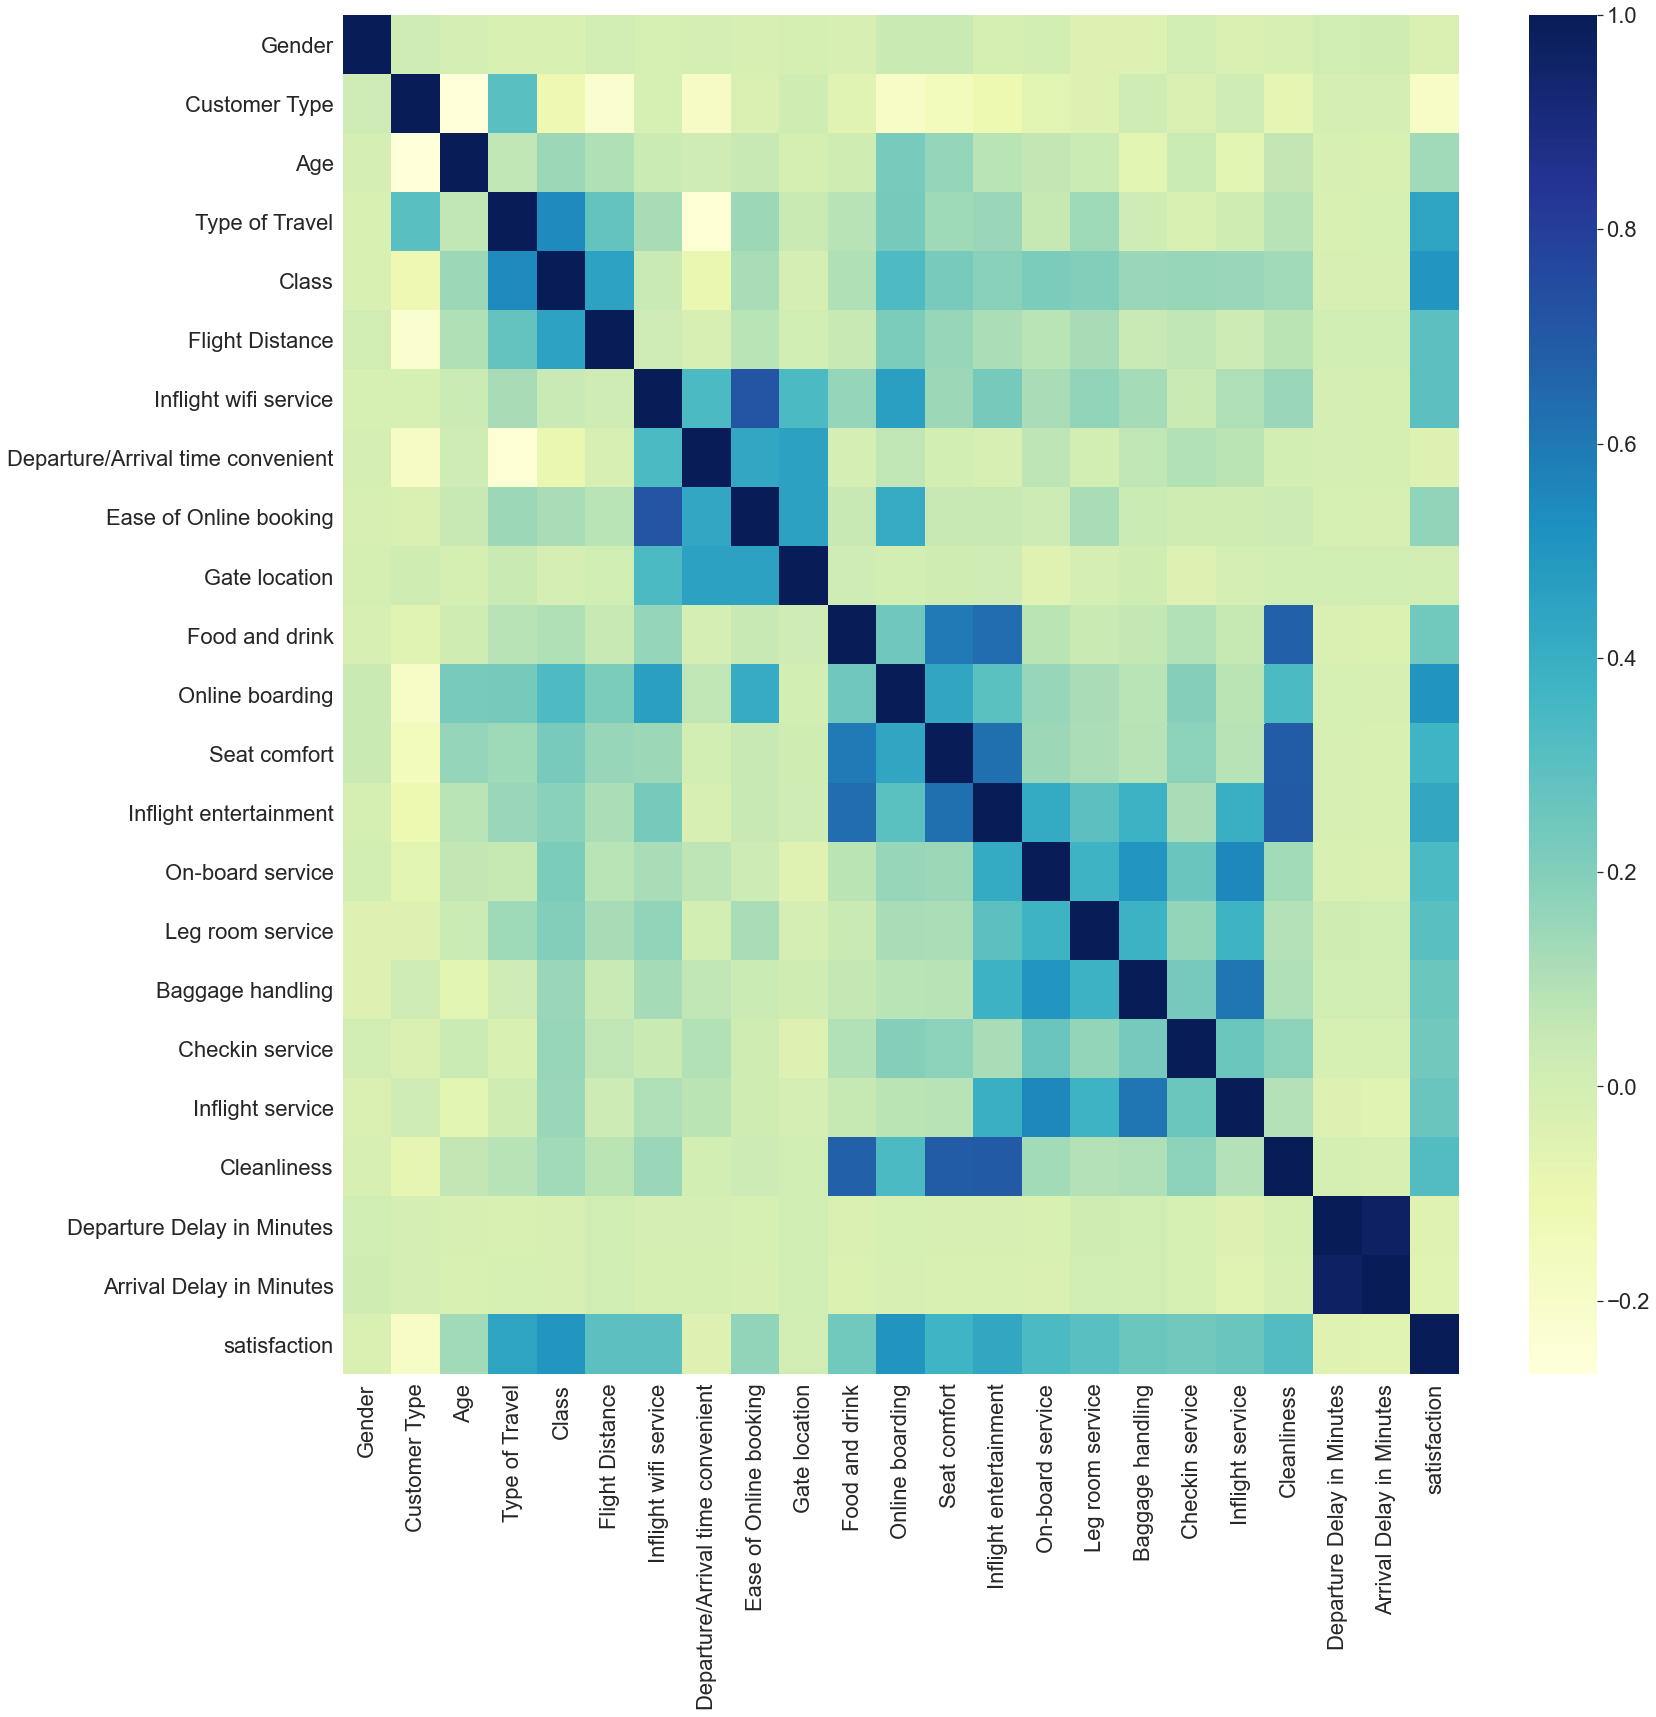
\includegraphics[width=0.8\textwidth]{corr_heatmap.png}
	  \caption{Correlation Heatmap of US Airline Passenger Dataset}
      \label{fig:corr_heatmap}
  \end{figure}

  \noindent The variables of the dataset are classified as follows:

  \begin{itemize}
    \item \textbf{Categorical Variables:} Gender, Customer Type, Type of 
      Travel, Satisfaction
    \item \textbf{Ordinal Variables:} Class, Inflight WiFi Service, Ease of Online
      Booking, Gate Location, Food and Drink, Online Boarding, Seat Comfort,
      Inflight Entertainment, On-Board Service, Leg Room Service, Baggage
      Handling, Check-in Service, Inflight Service, Cleanliness
    \item \textbf{Numerical Variables:} Age, Flight Distance, Departure Delay in
      Minutes
  \end{itemize}

  \noindent The categorical variables were dummy coded and the ordinal variable
  Class was recorded as shown in table \ref{table:airline_summary}. The
  remaining ordinal variables which measure different satisfaction levels were
  recorded using a Likert scale ranging from $1 - 5$. Many passengers did not
  answer all satisfaction level questions. These responses were recorded
  with a 0. Therefore, the range of values for the satisfaction level variables
  range from $0 - 5$. This encoding works well, as a 0 input in a linear pass
  function of a (graph) neural network will result in a 0 output value. This
  type of encoding allows us to deal with missing values for neural networks
  and other machine learning methods. Lastly, the numerical variables had to be
  normalized. The popular approach of standardizing the entire dataset was 
  unfortunately not possible, because it had to be ensured, that a 0 was 
  referred to as a missing response. Note, that a 0 for the numerical variables 
  does not correspond to a missing value. The normalizing function employed is
  defined as follows:

  \begin{equation}
    x' = a + \frac{(x - \min(x))(b - a)}{\max(x) - \min(x)}
    \label{eq:norm}
  \end{equation}

  \noindent In equation \ref{eq:norm}, $x$ refers to the unnormalized 
  variable and $x'$ refers to resulting normalized variable. $a$ defines 
  the lower bound of the normalization range and $b$ is the upper bound. The
  numerical variables were normalized withing the range 1-5 using equation
  \ref{eq:norm}. Now, all variables are within a similar range and different 
  scaling should no longer lead to a biasing behavior. \\

  \noindent In the following section, the graph generation process for the US
  Airline Passenger dataset is described in detail.

  \subsection{Graph Generation}
  \label{section:graph_gen}

  To create a graph from the US Airline Passenger Dataset, appropriate
  attributes must be selected for the MAG model. The selected attributes must be
  of the type such that realistic probabilities can be assigned. As an example, 
  it is difficult to assign link-affinity probabilities for people who gave 
  ratings regarding the "inflight wifi service". In this case one could assign 
  a probability that people who gave high ratings are more similar with 
  relative ease. However, does this then also translate to people not liking 
  the wifi-service being similar as well? Further, how do we assign 
  probabilities for people who are dissimilar? These considerations make the 
  selection of appropriate attributes difficult. It is therefore important to 
  select attributes for which realistic variables for all of the following
  three settings can be assigned:

  \begin{itemize}
    \item \textbf{Positive similar observations} (e.g. both observations like 
      the service)
    \item \textbf{Negative similar observations} (e.g. both observations 
      dislike the service)
    \item \textbf{Dissimilar observations} (Symmetric for undirected graphs, 
      can be asymmetric for directed graphs)
  \end{itemize}
 
  \noindent The attributes were selected using the above mentioned 
  considerations. The selected attributes with the corresponding link-affinity 
  probabilities are shown in table \ref{table:link_aff}.

  \begin{table}[h]
    \centering
    \begin{tabular}{|l||L|}
      \hline
      \textbf{Attribute Name} & \textbf{Link-Affinity Probabilities}\\
      \hline\hline
      Gender & 0.6, 0.4; 0.4, 0.6  \\\hline 
      Customer Type & 0.8, 0.5; 0.5, 0.8 \\\hline
      Age & 0.90, 0.80, 0.60, 0,40; 0.80, 0.90, 0.80, 0.60; 0.60, 0.80, 0.90,
      0.80; 0.40, 0.60, 0.80, 0.90 \\\hline
      Type of Travel & 0.80, 0.20; 0.20, 0.80 \\\hline
      Class & 0.85, 0.60, 0.45; 0.60, 0.85, 0.60; 0.45, 0.60, 0.85 \\
      \hline
    \end{tabular}
    \caption{Link-Affinity Matrices}
    \label{table:link_aff}
  \end{table}

  \noindent The probabilities in table \ref{table:link_aff} correspond to the
  rows of the link-affinity matrices up to the semi-colon. To give a better
  overview, the link-affinity matrix for age is shown explicitly as follows:

  \[ \Theta_{Age} = 
	\begin{pmatrix}
		0.90 & 0.80 & 0.60 & 0.40 \\
        0.80 & 0.90 & 0.80 & 0.60 \\
        0.60 & 0.80 & 0.90 & 0.80 \\
        0.40 & 0.60 & 0.80 & 0.90 \\
	\end{pmatrix}
  \] 

  \noindent Age was not only selected as an example as it is the largest
  link-affinity matrix, it also required some additional data transformation.
  The MAG model can only consider discrete variables which is why age had to be
  binned into discrete categories. Age was binned into 4 bins with 0 if age $<$ 
  26, 1 if 26 $\leqslant$ age $<$ 39, 2 if 39 $\leqslant$ age $<$ 50 and 3 if age
  $\geqslant$ 50. These bins were chosen according to the interquartile lengths 
  present in the distribution of the variable age. \\

  \noindent For assigning link-affinity probabilities there exist no clear rules 
  as to how these are to be defined. The article by Kim \& Leskovec 
  (\citeyear[p. 118]{kim2012multiplicative}) shows the 4 common structures of 
  homophily, heterophily, core-periphery and random for creating graphs. Given 
  the selected attribute data, the homophily setting was most appropriate for 
  all link-affinity matrices. In this setting, observations which are similar 
  have a higher probability of forming a connection compared to dissimilar 
  observations. The probabilities were assigned based on personal intuition and 
  trial and error. Several graphs were created using different probabilities, 
  where the probabilities shown in table \ref{table:link_aff} generated the most 
  reasonable graphs. There is however no exact science or selection criteria 
  which can be applied for selecting attributes and defining the link-affinity 
  probabilities. \\

  \noindent As mentioned in the previous section, a sub-sample of 6'000 
  observations was retrieved from the training dataset consisting of 103’904 
  observations. With this random sub-sample and the attributes shown in table
  \ref{table:link_aff}, the adjacency matrix for the 
  resulting graph, $G(V,E)$ was generated using algorithm \ref{algo:MAG}. The 
  random sub-sample was retrieved due to the computational cost involved for 
  applying algorithm \ref{algo:MAG}. Simulations involving creating graphs with 
  different random sub-samples suggest, that the random sub-samples are 
  representative for the entire dataset. This suggestion is supported when
  comparing the summary statistics of the sub-sample with the full-dataset. The
  generated graph is shown in figure \ref{fig:us_airline_graph}.

  \begin{figure}[h]
	  \centering
	  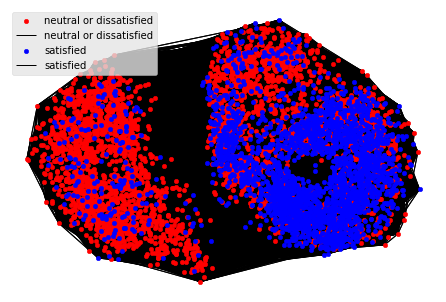
\includegraphics[width=0.7\textwidth]{us_airline_graph.png}
	  \caption{Graph of US Airline Passenger Dataset}
      \label{fig:us_airline_graph}
  \end{figure}
  
  \noindent The network shown in figure \ref{fig:us_airline_graph} show the
  emergence of two primary clusters. In addition one can see, that most satisfied 
  airline passengers appear to be grouped together in the right cluster. To 
  gain a deeper understanding of the dynamics involved in the network formation, 
  the nodes of the network are plotted excluding edges in figure
  \ref{fig:us_airline_nodes}.

  \begin{figure}[h]
	  \centering
	  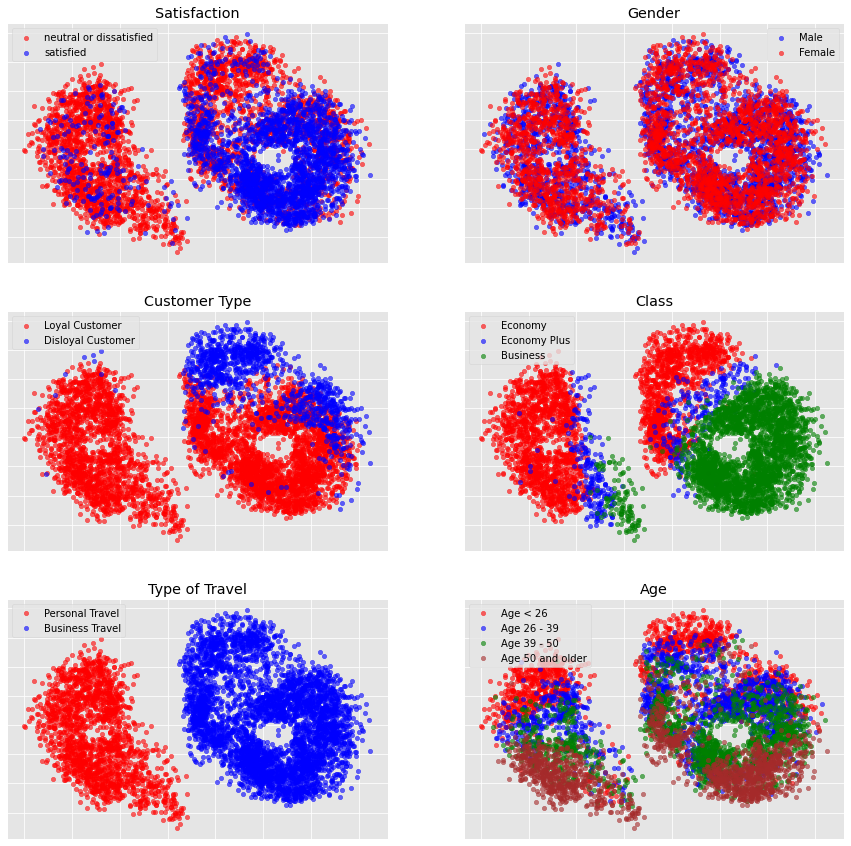
\includegraphics[width=0.8\textwidth]{us_airline_nodes.png}
	  \caption{Graph Nodes of US Airline Passenger Dataset}
      \label{fig:us_airline_nodes}
  \end{figure}

  \noindent Figure \ref{fig:us_airline_nodes} plots the nodes of the network
  for the label "Satisfaction" and the 5 attributes used for the graph
  generation. The transparency of the plot was set to $\alpha = 0.6$ to avoid 
  covering nodes during the graph plotting process. Figure
  \ref{fig:us_airline_nodes} reveals interesting associations. First it is
  shown, that a larger number of people traveling for business purposes are 
  satisfied compared to people traveling for personal reasons. This association
  becomes clear when comparing the satisfaction plot with the type of travel
  plot. In relative terms, only approximately 9.8\% of passengers traveling for 
  personal reasons were satisfied compared to business travelers with a 57.8\% 
  satisfaction rate. Interestingly, passengers traveling for business purposes
  hold somewhat expected characteristics such as:

  \begin{enumerate}
    \item Most business class passengers are satisfied. 
    \item Older passengers appear to be more satisfied which is largely
      associated with booking more business class tickets. The age plot however 
      reveals, that older passengers tend to be mostly satisfied even when 
      booking economy class.
    \item Most loyal customers book business class. There is some overlap where 
      loyal customers book economy class tickets. The reverse is true as well, 
      where a cluster of disloyal customers book business class. 
  \end{enumerate}
  
  \noindent Passengers traveling for personal reasons do not appear to adhere
  to the characteristics or associations shown for business travelers. The only
  distinctive character is, that almost all passenger traveling for personal
  reasons are loyal customers. This fact does however not appear to be
  associated with satisfaction. This appears to be a rather bizarre finding.
  Upon further reflection, this could point to a sampling bias of passengers
  traveling for personal reasons based on following considerations:

  \begin{enumerate}
    \item It makes sense, that almost only loyal passengers participated, as
      when traveling, most people do not participate in surveys. This is
      especially true for disloyal customers. Business travelers for comparison
      might give feedback due to company policies.
    \item It is common, that dissatisfied people are more likely to give
      feedback, while satisfied passengers are less likely to participate in
      the survey. Again, the data regarding business travelers might be more
      reliable here due to company mandated survey participation.
    \item Perhaps business travelers fly more frequently than passengers
      traveling for personal reasons. This could incentivize frequent business
      travelers to give feedback as they would benefit most of service
      improvements. Infrequent personal travelers might be less incentivized,
      as they are less affected by service improvements. 
  \end{enumerate}

  \noindent Last but not least, gender does not appear to form any distinguishable 
  clusters. For that reason, it was considered to omit this attribute for the 
  graph generation process. This was tested and the resulting graph yielded 
  a similar graph. The graph was however more spread out and the neighborhood 
  structures were less clear. In addition, the graph without gender did not 
  perform as well in the subsequent machine learning tasks. For those reasons, 
  gender was kept for the graph generation process. \\

  \noindent To provide some more context regarding the graph structure, some
  graph theoretical metrics are provided. The degree distribution as well as 
  the distributions of the centrality measures: eigenvector centrality, 
  closeness centrality and betweenness centrality are shown in 
  figure \ref{fig:centrality_measures}.

  \begin{figure}[h]
	  \centering
	  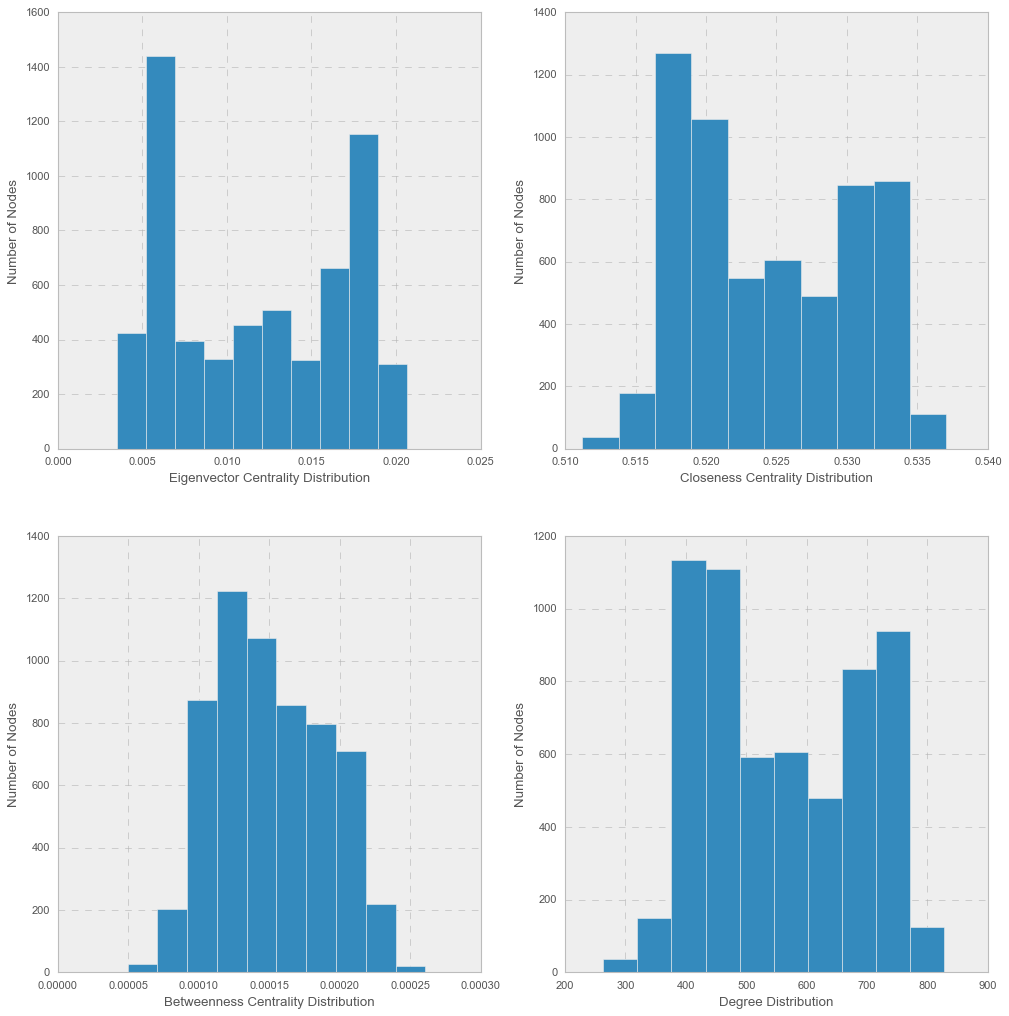
\includegraphics[width=0.7\textwidth]{centrality_measures.png}
	  \caption{Graph Statistics}
      \label{fig:centrality_measures}
  \end{figure}

  \noindent The network has a density of approximately 0.0933. This means that 
  9\% of the potential number of connections formed in the network.
  Nevertheless, when looking at the degree distribution histogram we can see, 
  that a all nodes have a large number of connections ranging between 263 -
  828 with an average of 559.63 connections. Further, the distribution has two
  modes which likely correspond to the two main clusters shown in figure
  \ref{fig:us_airline_nodes}. The eigenvector centrality distribution shows, 
  that all nodes have a very low centrality measure and therefore none of the 
  nodes appear to have a large impact in terms of eigenvector centrality. The 
  closeness centrality distribution shows, that all nodes have an average 
  closeness centrality ranging from 0.51 - 0.53. This means that every node is 
  similarly connected and has an average impact for disseminating information 
  across the network. Lastly, the betweenness centrality distribution reveals 
  that there are no bottle-necks through which information flows. \\

  \noindent As a reference point, it is important to compare the properties of
  the created graph to real world graphs. In our case, the most appropriate for
  comparison is a social network. Common structures of social networks are
  \citep{watts1998collective,newman2006structure,Newman2010,
  kim2012multiplicative}:

  \begin{enumerate}
    \item Degree distributions often follow a power law distribution
    \item Emergence of a giant connected component
    \item Core-periphery structure
  \end{enumerate}

  \noindent This power law degree distribution and emergence of a giant
  connected component creates network structures that have an onion
  (core-periphery) structure \citep[p. 121]{kim2012multiplicative}. This
  indicates, that most social networks have a few very highly connected nodes
  and many nodes with few connections. This creates a right skewed degree 
  distribution which also lead to a right skewed eigenvector centrality and
  closeness centrality distribution. For the betweenness centrality, we would
  also expect, that more central nodes in a core-periphery network structure
  would exhibit some bottle-neck properties for the central nodes. For that
  reason we would expect central nodes to have a higher betweenness centrality.
  When we look at the distributions in figure \ref{fig:centrality_measures}
  this does not correspond to the power law degree distribution and the effect
  this has on the centrality measures observed in real social networks. This
  indicates, that the graph created with the MAG method does not share the
  properties observed in real social networks. In order to generate a graph which
  shares the properties of real graphs, one would have to adapt the 
  link-affinity properties to the core-periphery setting as shown in figure
  \ref{fig:link-affinity}. Forcing this core-periphery structure is however not
  purposeful for this thesis. Further, the aim of this thesis is not
  necessarily to create realistic graphs rather than to create useful graphs 
  for graph machine learning. The results in chapter \ref{section:results}
  reveal, that the graph is indeed useful for graph machine learning. For that
  reason, the generated graph shown in this section is kept for further
  analysis. 

  \subsection{Stochastic vs. Deterministic MAG}
  \label{section:stoch_det}

  As addressed in section \ref{section:self_survey}, the question was raised 
  as to whether the MAG should form connections between observations
  stochastically or whether a deterministic threshold probability yields better 
  results. The first insight gained when investigating this question lies in 
  the fact, that the probability of two observations is generally very low. 
  When setting the threshold probability for a connection between two 
  observations $u$ and $v$ to 0.5, not a single connection was made. This makes 
  sense, as the probability for a connection decreases by design as the number 
  of attributes increases. This is implicitly shown in equation \ref{eq:MAG}, 
  where the product of probabilities is bound to decrease. For this reason, it 
  is suggested to limit the number of attributes to $K=\rho\log_{2}N$ for some 
  constant $\rho$ \citep[p. 122]{kim2012multiplicative}. The number of 
  attributes were selected accordingly such that $K\leqslant\log_{2} N$. The 
  US Airline Passenger dataset was used to generate a deterministic graph. The 
  threshold probability for a connection was set to 0.2 in the MAG model. The 
  MAG yielded several disconnected graphs which were for the most part 
  clustered according to their group memberships. Figure \ref{fig:det_MAG} 
  shows the graphs for the label and the attributes, where the edges were 
  removed. The subgraphs are unfortunately plotted small, however all subgraphs 
  combined include all 6'000 nodes. The plots are meant to provide a high-level 
  overview of the generated graphs. 

  \begin{figure}[h]
		\centering
		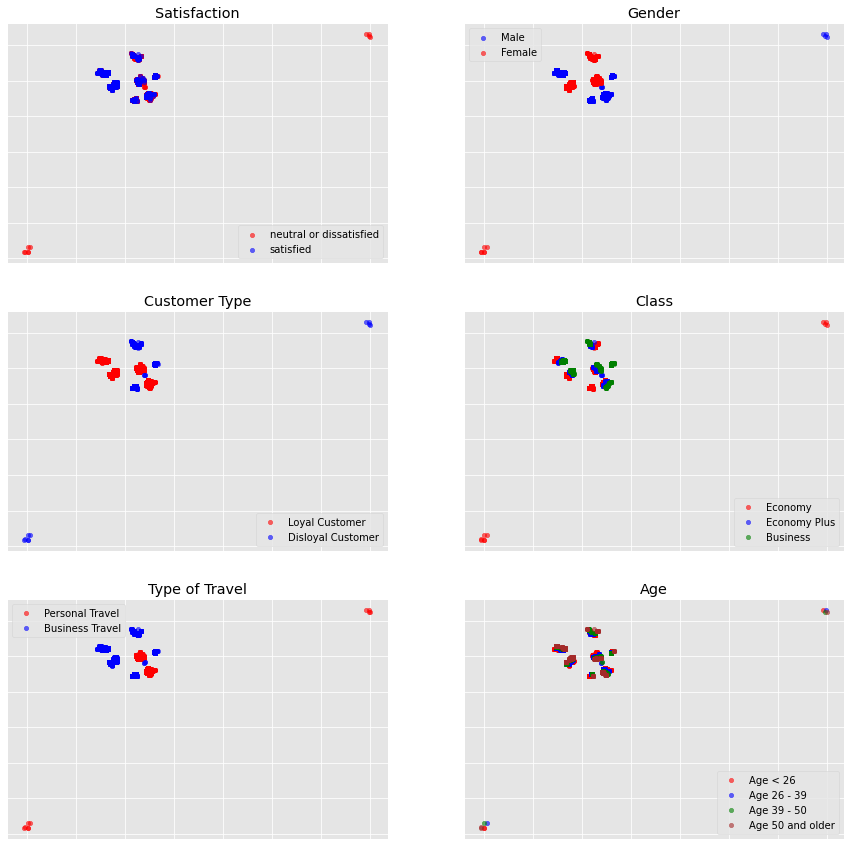
\includegraphics[width=1.0\textwidth]{deterministic_MAG.png}
		\caption{Deterministic MAG graph}
        \label{fig:det_MAG}
  \end{figure}

  \noindent The deterministic MAG model crates disconnected graphs which form 
  clusters based on node similarities. In terms of performance, the accuracy 
  and loss behavior of both the deterministic- and stochastic generated graphs 
  are virtually identical. This was true for all three datasets considered in 
  this thesis. For the purpose of visualization, stochastic graphs appear
  to be more useful, as one can identify the different cluster on a single
  connected graph. For this reason, the stochastic graph generation process is 
  kept. Nevertheless, deterministic graph generation appears to be useful if 
  one wants to separate nodes in to more homogeneous graphs. These 
  graphs could then be used for subsequent machine learning tasks with a cluster 
  specific task in mind. The clusters further could provide information as to 
  which clusters tend to be more or less satisfied. This is an area which could 
  be interesting for future research.
  

  \label{section:data}

  %\chapter{Conclusion}
  %
  This chapter includes the conclusion and provides an outlook for future
  research.

  \section{Conclusion}
  \label{section:conclusion}

  The aim of this thesis is to assess to what extent semi-synthetic graphs based 
  on real feature data are useful for machine learning. This aim corresponds to
  the research question stated in section \ref{section:research_topics}. The
  results for answering this question are mixed and are based on the data
  presented in chapter \ref{section:data}, the results of chapter
  \ref{section:results} and the discussion in chapter \ref{section:discussion}.
  \\

  \noindent Graph machine learning on the graph created from the Bank 
  Telemarketing dataset fails to overcome the problem of unbalanced labels. It 
  however yields similar results in terms of accuracy as the standard machine 
  learning models. In addition it is shown, that if a network structure can be 
  created which corresponds to the label, that the problem of unbalanced label 
  data could be overcome. \\

  \noindent GraphSage performs well for the US Airline Passenger dataset and
  is second only to the random forest classifier in terms of accuracy. As
  discussed, following the principle of Occam's razor, the good results for the
  GraphSage model must be taken with a grain of salt. For the purpose of
  gaining customer insights, simpler models such as ANN, SVM or AdaBoost provide
  only marginally inferior results and are more practical and thus preferable
  for this setting. Given similar results for more sensitive applications such
  as medicine, the GraphSage model could be preferred as even marginal
  performance improvements can be of utmost importance. In short, the GraphSage
  yields competitive results in terms of accuracy, the results are however not
  superior enough to necessarily warrant the complex graph generation process
  and model complexity of GraphSage. Lastly, the graph convolutional network and
  Node2Vec are not successful for the given classification task. For that
  reason more recent graph machine learning models should be tested and/or new 
  models should be developed to expand the possibilities of graph machine 
  learning.\\

  \noindent The perhaps most interesting result is provided by the US Airline
  Passenger graph plots shown in figure \ref{fig:us_airline_nodes}. The MAG 
  model successfully generates neighborhoods within the graph, where the nodes 
  are grouped according to their similarity which respects the similarities 
  between all attributes. This observation is further confirmed by the scatter 
  plots shown in figure \ref{fig:node2vec}. The graphs and the scatter plots
  make it possible to visually interpret the relationships within the data. 
  Standard scatter plots using the feature data do not allow for the generation 
  of such insightful graphs/plots. \\

  \noindent To summarize and provide an answer to the research question, it is
  shown that yes, semi-synthetic graphs can be useful for machine learning in a
  classification setting. The graph machine learning models are shown to be 
  competitive and could potentially even provide a solution for overcoming the 
  difficulties associated with unbalanced label data. This however requires the 
  availability of a graph with a structure which corresponds to the label. The 
  usefulness of semi-synthetic graphs are limited by the complexity associated 
  with generating graphs and the general complexity of graph machine learning 
  models. The graph based models further fail to outperform the standard machine 
  learning methods and are ranked anywhere between the second to fifth best 
  method depending on how one weights the trade off between model complexity 
  and accuracy. Based on this, the hypotheses presented in section
  \ref{section:research_topics} can be answered as follows: \\

  \noindent\textbf{H1:} Graph machine learning using semi-synthetic graphs fail
  to outperform standard machine learning methods. This hypothesis is thus
  rejected. \\

  \noindent\textbf{H2:} Graph machine learning is shown to be a competitive
  strategy with competitive results in line with the results shown for the
  standard machine learning methods. This hypothesis is not rejected.

  \section{Outlook}

  The discussion in chapter \ref{section:discussion} and the conclusion in section
  \ref{section:conclusion} provides interesting topics for future research.
  These topics include graph generation, cluster analysis on graphs and graph 
  machine learning models. 

  \paragraph{Graph Generation} \mbox{}
  
  \noindent Creating semi-synthetic graphs using the MAG method is shown to be a 
  viable method. The graph is however sensitive to attribute selection and 
  setting appropriate link-affinity probabilities. A fist step for resolving
  this issue was introduced by \cite{kim2011modeling} as a follow-up to their
  MAG model. In this paper they propose a reverse model, in which given a real
  graph, the attributes and the link-affinity probabilities are estimated such 
  that the attributes and link-affinity probabilities generate the observed real
  graph. This is however only a partial solution to the task given for this
  master's thesis. The estimated attributes do not correspond to real 
  attributes/features. In this model, the attributes are estimated to fit the 
  graph. An interesting topic for future research would be to develop a model 
  that generates a semi-synthetic graph based on attributes which at the same
  time optimizes link-affinity probabilities such that the resulting graph
  adheres to network properties observed in real graphs. Perhaps these more
  realistic graph properties can improve the performance for graph machine
  learning. This is an area worth consideration as especially the degree
  distribution and centrality measures shown in figure 
  \ref{fig:centrality_measures} force graph machine learning models to consider
  a large number of neighbors. In addition, even when sampling, the
  neighborhood is bound to always have the same size, given the range of the
  degree distribution shown in figure \ref{fig:centrality_measures}. This is a
  potential limiting factor for graph machine learning, as it potentially makes
  it more difficult to distinguish- and make use of different structures
  withing the graph.

  \paragraph{Cluster Analysis on Graphs} \mbox{}

  \noindent The graph plots shown in figure \ref{fig:us_airline_nodes} reveal,
  that semi-synthetic graphs can be excellent tools for visualizing data. The
  amount of useful information provided for interpreting the data is a welcome
  and unexpected result. For understanding the relationships between the
  attribute data and the label, the graph plots yielded the most useful
  information for identifying relationships within the data. An interesting
  topic for future research could be to assess how common clustering methods
  such as k-means, fuzzy clustering or CLIQUE could be used for analyzing
  graphs. Perhaps better and more graph centric methods could be developed. An
  excellent overview of existing graph clustering methods is provided by
  \cite{zhou2020graph}. Their article can be used as an initial reference point
  for identifying new applications of existing graph clustering methods or for 
  developing new models.

  \paragraph{Graph Machine Learning Models}\mbox{}

  \noindent Graph convolutional networks and GraphSage are selected for this
  thesis as they are probably the two most well-known GNNs. There are however 
  newer and more sophisticated models such as \ac{gat} \citep{velivckovic2018graph} 
  or \ac{gin} \citep{xu2019powerful}. \\

  \noindent GAT models have the ability of identifying more- or 
  less important neighbors in the graph. This is a useful ability and has been 
  shown to improve performance in some cases. This ability is unfortunately 
  most likely limited by the very large number of neighbors present in the US Airline 
  Passenger graph as shown in figure \ref{fig:centrality_measures}. For that
  reason, more realistic graphs with smaller number of degrees should be
  generated as suggested in the previous graph generation paragraph. \\

  \noindent GIN models are very well suited for distinguishing structures 
  within the graph. The authors \cite{xu2019powerful} present the general GIN
  framework which can accept any type of features as inputs whilst ensuring
  that the aggregation function is injective. Given the injective aggregation
  strategy, it is shown that the GIN can be as expressive at distinguishing
  graph structures as the Weisfeiler-Lehman graph isomorphism test 
  \citep{weisfeiler1968}. Again, for such a model to work best, the number of
  degrees would most likely need to be smaller than currently present in the
  graph of the US Airline Passenger dataset. Given the large number of degrees,
  the neighborhoods of every node are currently of the same size when using the
  sampling strategy outlined for the GraphSage model. \\

  \noindent Given a more realistic graph with a smaller number of degrees, it
  would be interesting to develop and assess, whether a new method which
  includes the attention mechanism of the GAT network with the isomorphic 
  capabilities of the GIN method could be of use. This new model could for
  instance be tested on well understood benchmark graphs such as Cora
  \citep{mccallum2000automating} or Citeseer \citep{giles1998citeseer}. 




  %%% endmatter
  \bibliography{bibliography.bib} 

  \appendix
  
  %\chapter{Appendix Title}
  %
  \section{Pairplot Feature Data}
  \label{App:pairplot}
  
  The pairplot of the feature data of the US Airline Passenger Data is shown in
  figure \ref{fig:pairplot_feature}.

  \begin{figure}[h]
		\centering
		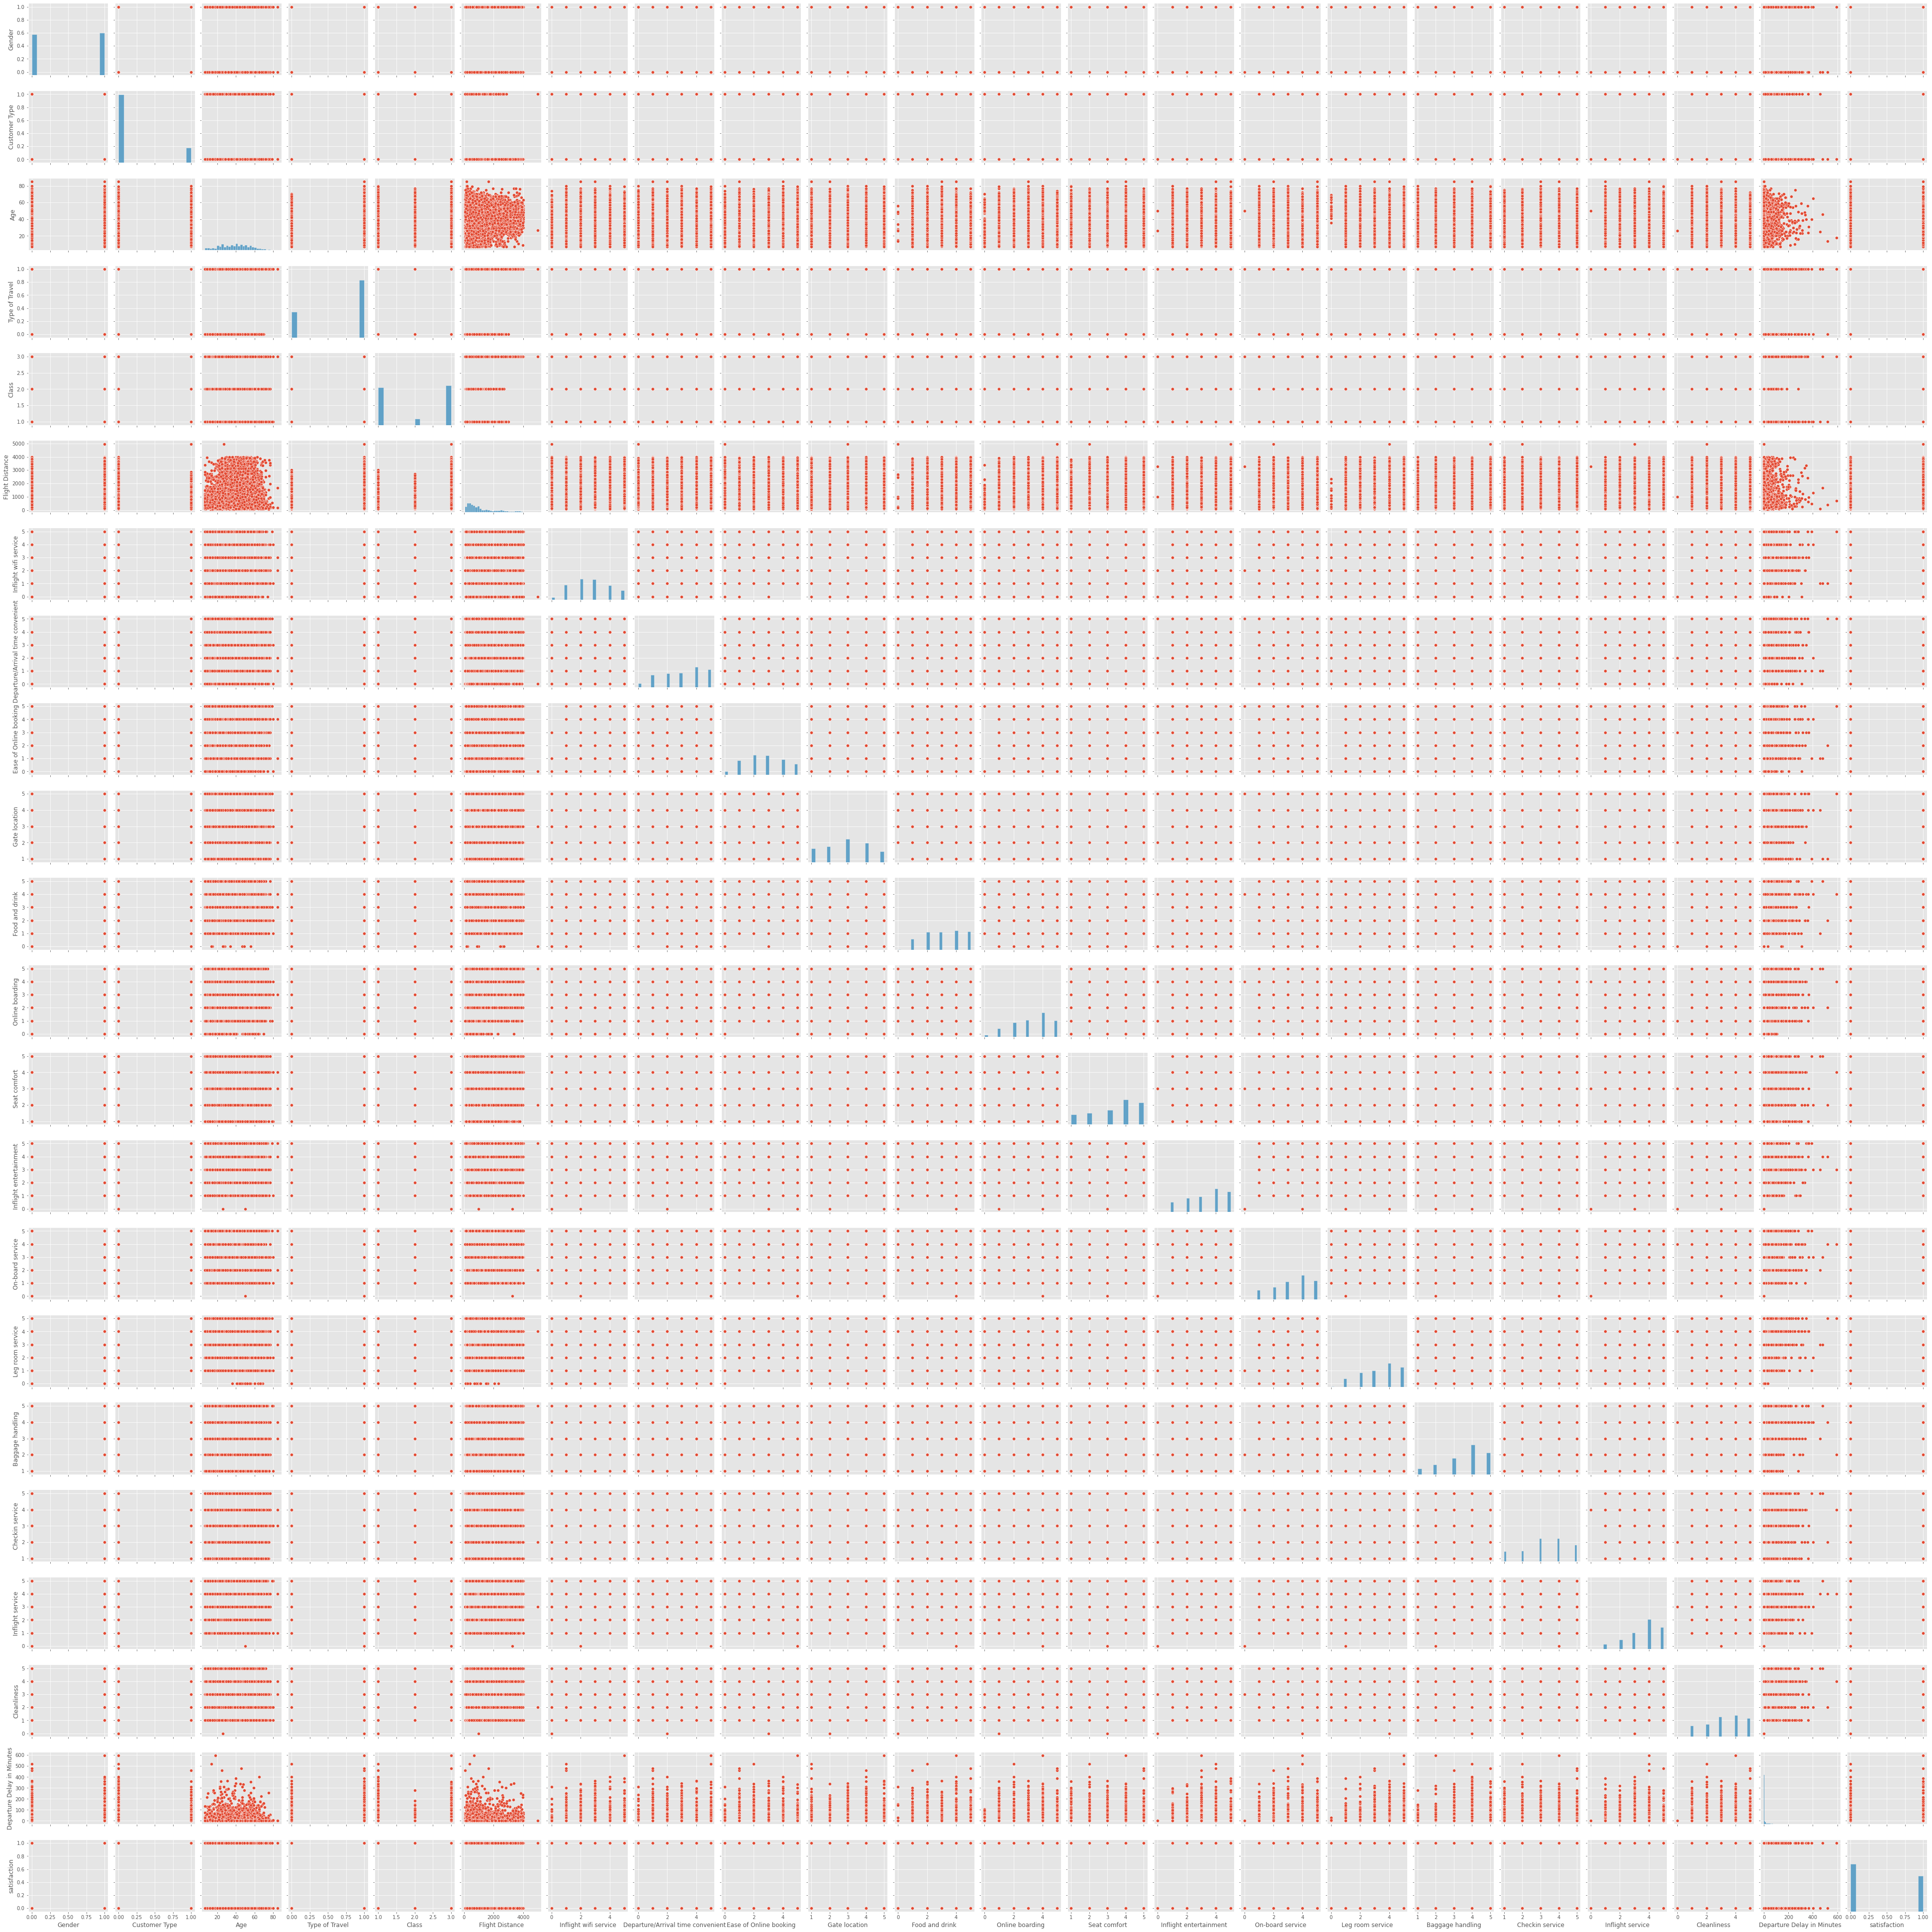
\includegraphics[width=0.9\textwidth]{pariplot_feature_data.png}
		\caption{Pairplot Feature Data US Airline Passenger Data Set}
        \label{fig:pairplot_feature}
  \end{figure}


\end{document}

